% Create a Table of Contents in Beamer
\documentclass[10pt,t]{beamer}
% Theme choice:
\usetheme{Singapore}
\useoutertheme{sidebar}
\usecolortheme{seahorse}
\setbeamercolor{titlelike}{bg=white}
\setbeamercolor{frametitle}{bg=white}
%\setbeamertemplate{frametitle}[default][left]
\setbeamertemplate{navigation symbols}{}

\usepackage{graphicx}
\usepackage{amsmath}
\usepackage{amsfonts}
\usepackage{amssymb}
\usepackage{amsthm}
\usepackage{ulem}
\usepackage{listings}

% Title page details: 
\title{Chapter 1c: Prediction in Linear Regression} 
\author{Taylor Okonek \& Charlie Wolock}
\date{\today}


\begin{document}
	% Title page frame
	\begin{frame}
	\titlepage 
\end{frame}

\begin{frame}{Learning objectives}
By the end of Chapter 1c, you should be able to:

\vspace{0.3cm} 
\begin{itemize}
	\item Understand and explain the difference between the scientific goals of prediction vs. inference
	\item Be able to compute fitted values in \texttt{R} and by hand
	\item Understand the importance of training vs. testing data, and how to create training and testing datasets in \texttt{R}
	\item Determine the predictive accuracy of a linear regression analysis using $R^2$ and mean squared error (MSE)
	\item Use $R^2$ and MSE to choose a prediction model
\end{itemize}
\end{frame}

% Outline frame
\begin{frame}{Outline}
\tableofcontents
\end{frame}

\AtBeginSection[ ]
{
\begin{frame}{Outline}
\tableofcontents[currentsection]
\end{frame}
}

% Presentation structure
% Prediction vs. Inference - difference in goals
% Fitted values review & examples - in R and by hand
% Training and testing data
% Measures of prediction accuracy
% - R^2
% - MSE
% Bias-variance tradeoff


\section{Prediction vs. Inference}

\begin{frame}{Prediction vs. Inference}
So far in this course, our goal has been to estimate the association between a predictor of interest and our outcome.

\vspace{0.3cm}

In Chapter 1b, we discussed the potential need to adjust for additional variables in our regression model (confounders, precision variables, effect modifiers). The inclusion of additional variables was motivated by scientific questions about \textit{association}, which led us to conduct \textit{statistical inference}.

\vspace{0.3cm}

When our scientific question involves \textit{prediction}, we have a different goal in mind: develop an algorithm based on current data that, when we plug in future data, predicts the outcome well.
\end{frame}

\begin{frame}{Prediction vs. Inference}
In loose terms:
\vspace{0.3cm}

\textcolor{blue}{Prediction:} using a model to predict outcomes for new data points

\vspace{0.3cm}

\textcolor{blue}{Inference:} understanding the relationships between variables (typically a predictor of interest and an outcome)
\end{frame}

\begin{frame}{Inference: scientific questions}
With inference, we are able to answer questions such as\dots

\vspace{0.3cm}

\begin{itemize}
	\item Are individuals with a specific genetic variable more susceptible to certain diseases later in life?
	\item Is there an association between access to antenatal clinics and maternal mortality in rural areas?
	\item Was a certain public health intervention associated with improved health outcomes for a community?
	\item Is a new vaccine effective at reducing the risk of getting a disease, or perhaps a severe case of the disease?
\end{itemize}

\end{frame}

\begin{frame}{Prediction: scientific questions}
With prediction, we are instead interest in questions such as\dots

\vspace{0.3cm}

\begin{itemize}
	\item How do predict risk of type II diabetes based on an individual's medical history?
	\item Can we accurately classify tumors in the central nervous system?
	\item What is the under-5 mortality rate at the state level for a country where we have no reliable census or vital registration data?
	\item Based on the videos a person has watched on YouTube, can we give them accurate suggestions for videos they would like to watch next?
\end{itemize}

\vspace{0.3cm} \pause

* questions like the last one are asked by companies all the time, including YouTube, TikTok, Netflix, or any company that provides some form of media or involves targeted advertising 
\end{frame}


\section{Fitted values}

\begin{frame}{Fitted values}
How do we actually use a model to \textit{predict} something? We use fitted values!

\vspace{0.3cm}

From Chapter 1a:

\vspace{0.3cm}

\textcolor{blue}{Fitted value}: the value of the response predicted from your regression \pause

\vspace{0.3cm}

Consider the linear regression model
$$
E[Y \mid X_1, \dots, X_p] = \beta_0 + \beta_1 X_1 + \dots + \beta_p X_p
$$

If we fit this model, we obtain coefficient estimates $\hat{\beta}_0, \dots \hat{\beta}_p$, and we can plug them into our regression equation to get fitted values $\hat{Y}$:
$$
\hat{Y} = \hat{\beta}_0 + \hat{\beta}_1 X_1 + \dots + \hat{\beta}_p X_p
$$

\end{frame}

\begin{frame}{Fitted values}
Each observation in our dataset gets a fitted value, based on their covariates values $X_1, \dots, X_p$. If we denote each observation by $i = 1, \dots, n$ for $n$ total observations, we can write these fitted values as
$$
\hat{Y}_i = \hat{\beta}_0 + \hat{\beta}_1 X_{i, 1} + \dots + \hat{\beta}_p X_{i, p}
$$

In two dimensions, fitted values are not too difficult to visualize (as we will do on the next slide). In higher dimensions (i.e., when we have more than one covariate in our model), fitted values are less easy to visualize.

\vspace{0.3cm}

Fitted values \textit{are} the predicted values (predictions) for each observation in our dataset!

\end{frame}

\begin{frame}{Fitted values: Visualizing in two dimensions}
In two dimensions (where we have only one predictor $X_1$), we can visualize fitted values on a scatter plot:
\vspace{0.3cm}

\centering 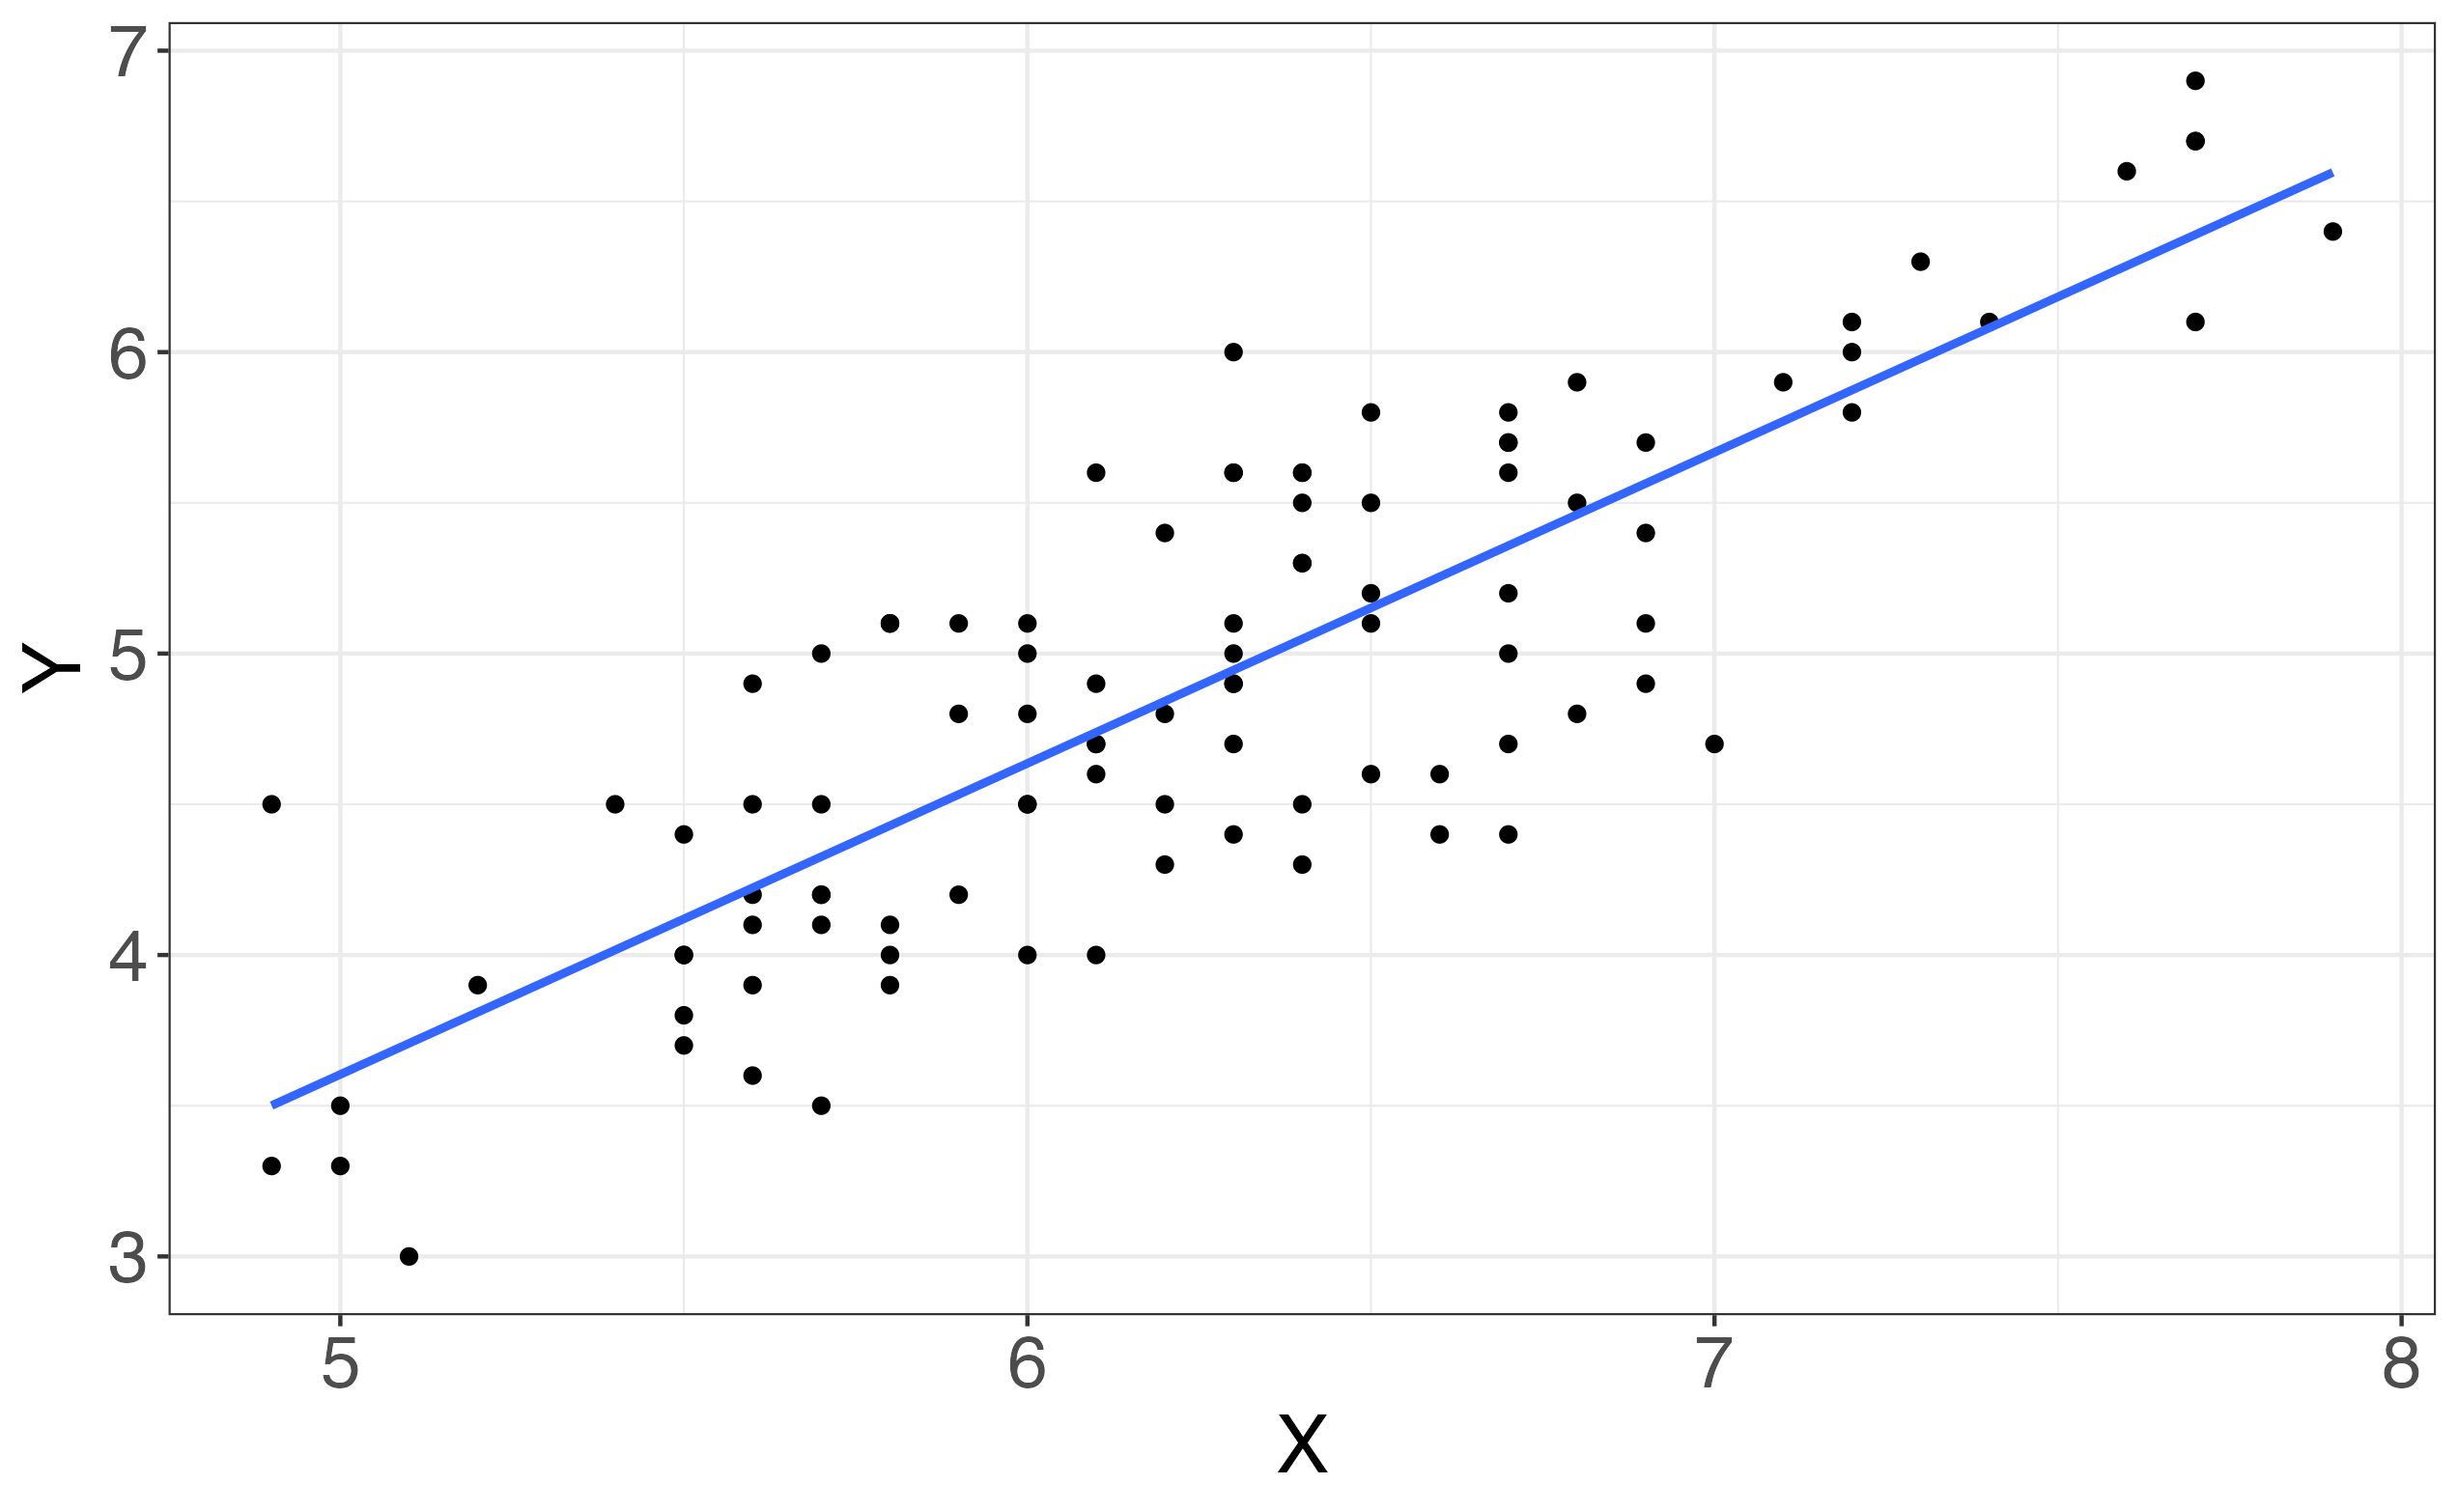
\includegraphics[scale=0.4]{fitted_vals1.png}
\end{frame}

\begin{frame}{Fitted values: Visualizing in two dimensions}
In two dimensions (where we have only one predictor $X_1$), we can visualize fitted values on a scatter plot:
\vspace{0.3cm}

\centering 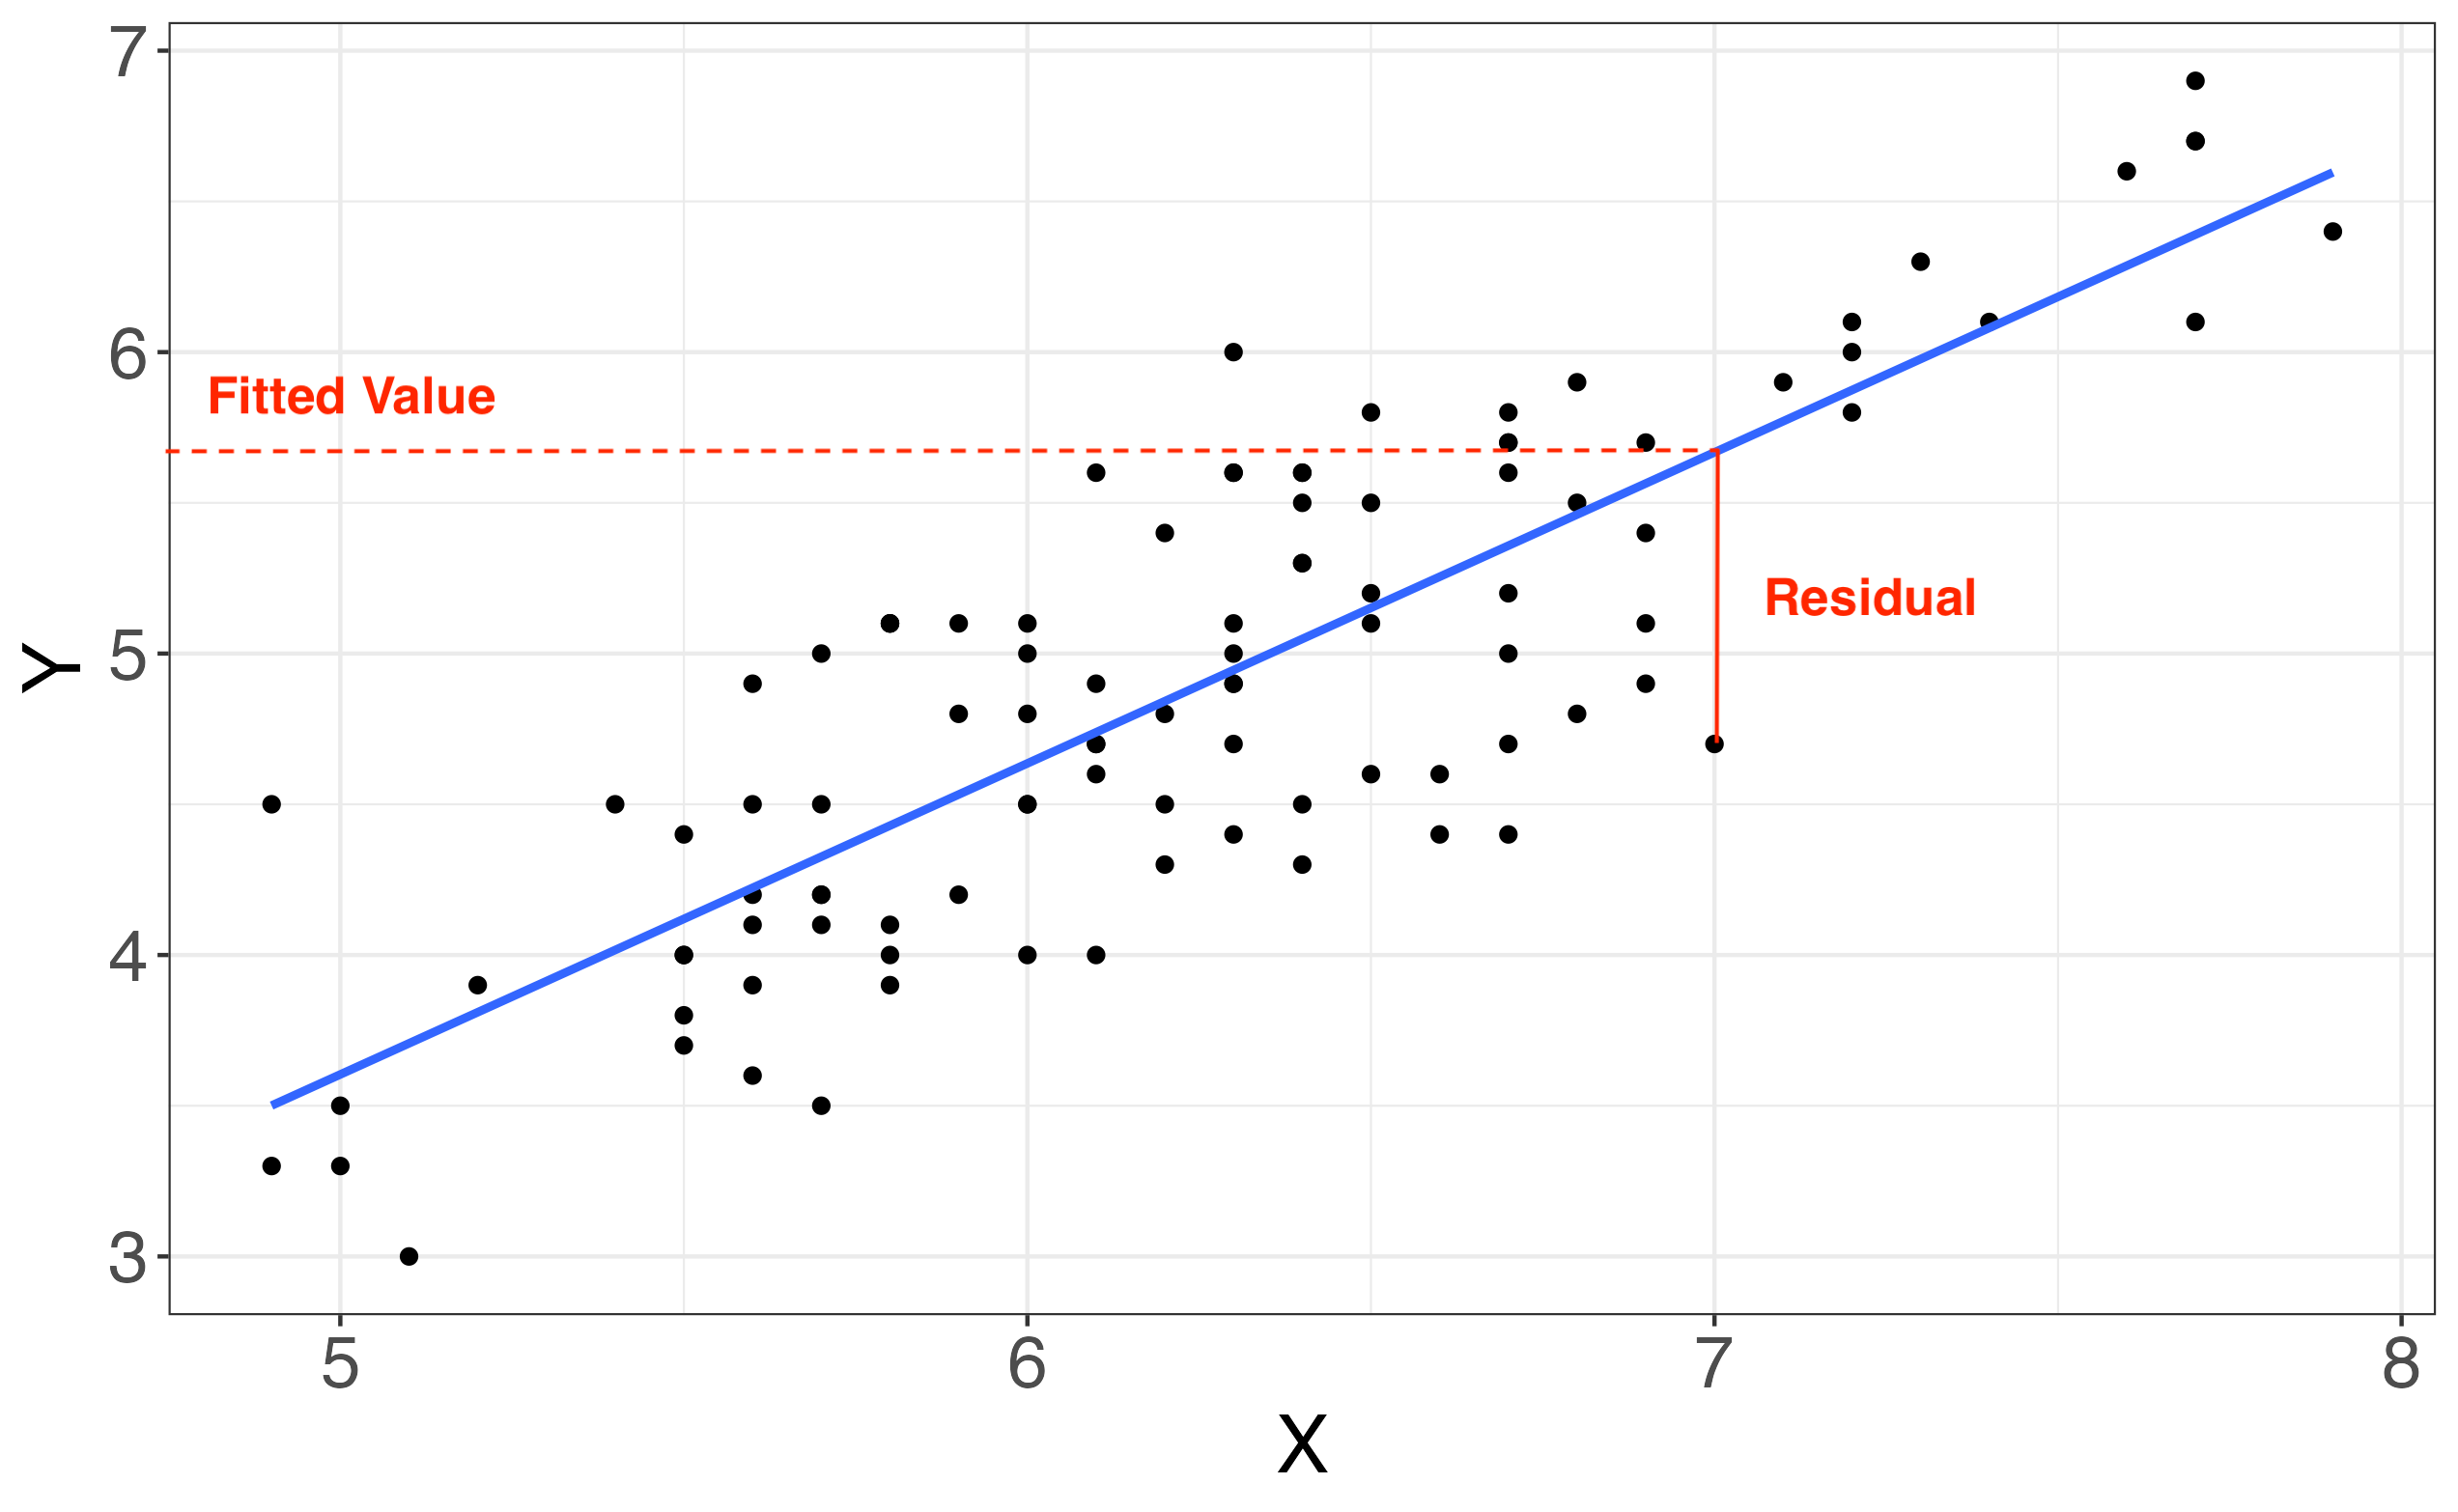
\includegraphics[scale=0.4]{fitted_vals2.png}
\end{frame}

\begin{frame}{Fitted values and prediction}
Fitted values allow us to obtain predictions for each observation in our dataset. Suppose we suddenly get covariate data ($X_1, \dots, X_p$) for a new observation, but we do not know their outcome $Y$. 

\vspace{0.3cm} 

\textcolor{blue}{Question:} Without re-fitting our linear regression model, how can we obtain a prediction for this observation based on their covariates? \pause

\vspace{0.3cm}

We can plug their covariates into our regression equation! If our dataset already has $n$ observations, we can denote this new observation as the $(n + 1)$'th observation, and write
$$
\hat{Y}_{n + 1} = \hat{\beta}_0 + \hat{\beta}_1 X_{(n + 1), 1} + \dots + \hat{\beta}_p X_{(n + 1), p}
$$

We can calculate by $\hat{Y}_{n + 1}$ by hand or in \texttt{R}, and we'll see examples of both.

\end{frame}

\begin{frame}{Prediction: Example in \texttt{R}}

Suppose we want are interested in predicting a baby's birthweight based on birth parent's age, marital status, whether or not they smoke during pregnancy, and weight prior to pregnancy. We can fit the appropriate regression model in \texttt{R}:

\vspace{0.2cm}

\centering 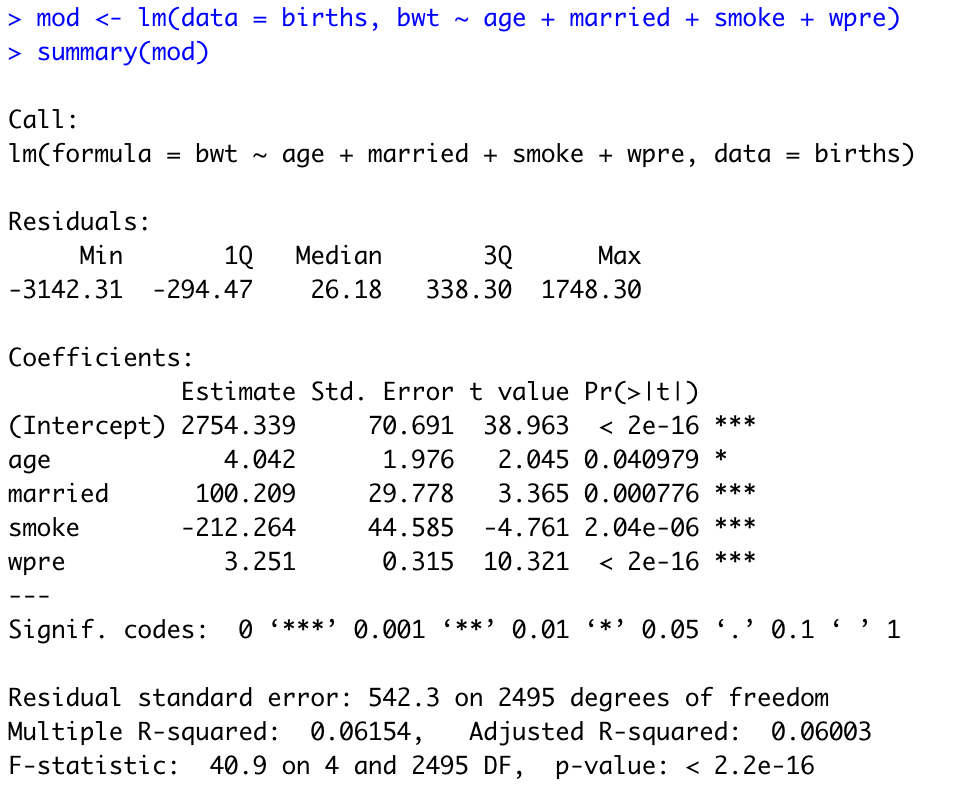
\includegraphics[scale=0.35]{predict_reg.png}
\end{frame}

\begin{frame}{Prediction: Example in \texttt{R}}
Extracting the coefficient estimates from this model and plugging them into our regression equation, we get
\begin{align*}
\hat{Y} = & 2754.339 + 4.042 \times \text{age} + 100.209 \times \text{married} \\
& - 212.264 \times \text{smoke} + 3.251 \times \text{wpre} 
\end{align*} \pause

What is our best estimate of a baby's birthweight born to a birth parent who is 25 years old, married, does not smoke, and weighed 150 pounds prior to pregnancy? \pause

\begin{align*}
\hat{Y} = & 2754.339 + 4.042 \times 25 + 100.209 \times 1 \\
& - 212.264 \times 0 + 3.251 \times 150  \\
& = 3443.223 \text{ grams}
\end{align*}

\end{frame}

\begin{frame}{Prediction: Example in \texttt{R}}
Extracting the coefficient estimates from this model and plugging them into our regression equation, we get
\begin{align*}
\hat{Y} = & 2754.339 + 4.042 \times \text{age} + 100.209 \times \text{married} \\
& - 212.264 \times \text{smoke} + 3.251 \times \text{wpre}
\end{align*}

What is our best estimate of a baby's birthweight born to a birth parent who is 15 years old, unmarried, smokes, and weighed 120 pounds prior to pregnancy? \pause

\begin{align*}
\hat{Y} = & 2754.339 + 4.042 \times 15 + 100.209 \times 0 \\
& - 212.264 \times 1 + 3.251 \times 120  \\
& = 2992.807 \text{ grams}
\end{align*}

\end{frame}

\begin{frame}{Prediction: Example in \texttt{R}}
Extracting the coefficient estimates from this model and plugging them into our regression equation, we get
\begin{align*}
\hat{Y} = & 2754.339 + 4.042 \times \text{age} + 100.209 \times \text{married} \\
& - 212.264 \times \text{smoke} + 3.251 \times \text{wpre}
\end{align*}

What is our best estimate of a baby's birthweight born to a birth parent who is 80 years old, married, does not smoke, and weighed 1000 pounds prior to pregnancy? \pause

\begin{align*}
\hat{Y} = & 2754.339 + 4.042 \times 80 + 100.209 \times 1 \\
& - 212.264 \times 0 + 3.251 \times 1000  \\
& = 6428.78 \text{ grams}
\end{align*}

* 6428.78 grams is approximately 13.3 pounds

\end{frame}

\begin{frame}{Prediction: extrapolation}
Our birthweight estimate for a birth parent who is 80 years old, married, does not smoke, and weighed 1000 pounds prior to pregnancy was 13.3 pounds. 13.3 pounds is not unheard of for a baby, but is very large.

\vspace{0.3cm}

\textcolor{blue}{Question:} Within our dataset, the oldest observed individual was 46 years old, and the individual with the highest pre-pregnancy birthweight was 350 pounds. Is it reasonable to make a prediction for an individual with covariate values so far outside of our dataframe? \pause

\vspace{0.3cm}

\textcolor{blue}{Answer:} It depends! If we believe that the observed linear relationship holds for covariate values even outside of those observed in our dataframe, then we may be okay. However, we have no way of knowing from our data whether or not the linear relationship holds for covariate values outside of our dataframe, because we don't observe them! 

\vspace{0.3cm}

\small Predicting values outside of the range of our observed data is known as \textcolor{blue}{extrapolation}, and is unreasonable to do in many scientific settings.

\end{frame}

\begin{frame}{Prediction: Example in \texttt{R}}
Rather than calculate predictions by hand, it is often useful to do this in \texttt{R}, and we can make predictions for more than one observation at a time. As in Chapter 1a to obtain fitted values for our observed data, we can use the \texttt{predict} function to get fitted values for new data as well.

\vspace{0.3cm}

To get fitted values for our observed data, we just call the \texttt{predict} function on our modeling object \texttt{mod} (where \texttt{mod} is the output of a regression model):

\vspace{0.3cm}

\texttt{fitted\_vals <- predict(mod)}
\end{frame}

\begin{frame}{Prediction: Example in \texttt{R}}
To get fitted values for new data, we use the \texttt{newdata} argument inside of \texttt{predict}:

\vspace{0.3cm}

\texttt{new\_df <- data.frame(...)} \\
\texttt{fitted\_vals <- predict(mod, newdata = new\_df)}

\vspace{0.3cm}

where \texttt{new\_df} is a dataframe that contains columns for all covariates in your model.

\end{frame}

\begin{frame}{Prediction: Example in \texttt{R}}
Earlier we calculated by hand our best estimate of a baby's birthweight born to a birth parent who is 25 years old, married, does not smoke, and weighed 150 pounds prior to pregnancy. In \texttt{R}, we can use the following code:

\vspace{0.3cm}

\begin{figure}
	\centering 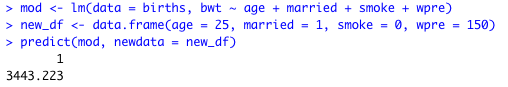
\includegraphics[scale=0.5]{newdata_example.png}
\end{figure}

\vspace{0.3cm}

\texttt{new\_df} is a dataframe containing a single row (one observation), for someone who is 25 years old, married, does not smoke, and weighed 150 pounds prior to pregnancy. It does all of the math for us!

\end{frame}

\begin{frame}{Prediction: Example in \texttt{R}}
We can also make predictions for multiple observations at the same time. For example, we can make predictions for all three of our examples from earlier using just a few lines of code:

\vspace{0.3cm}

\centering 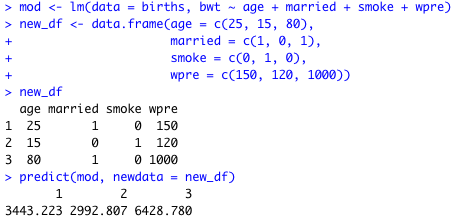
\includegraphics[scale=0.5]{newdata_example2.png}

\end{frame}

% could include a slide about thinking about which variables you can include in your model (i.e. not sex of child if we're predicting birthweight because not everyone knows the sex of their child before birth)

\section{Training and testing data}

\begin{frame}{Training and testing data}
Now that we are able to make predictions for new observations, we may be wondering how to tell whether or not we are predicting new observations \textit{well}. If our predictions are bad, they are not going to be particularly useful!

\vspace{0.3cm}

We care about ensuring that predictions are good for \textit{new observations}, rather than ensuring predictions are good for observations we have already observed. If we've already observed outcomes for certain individuals, we have no need to predict their outcomes (this would be redundant). Thus, we want to make sure our predictive model performs well on \textit{new} data, sometimes referred to as \textcolor{blue}{out-of-sample} data.

\vspace{0.3cm}

You may be wondering, how do we assess our model's performance on data that we have not yet collected?
\end{frame}

\begin{frame}{Training and testing data}
In practice, since we clearly do not have access to data that we have not yet collected, we instead pretend that some of the data we have in fact observed is ``new," and we try to accurately predict the observed outcomes on those ``new" observations. This involves splitting our dataset into \textcolor{blue}{training} and \textcolor{blue}{testing} data.

\vspace{0.3cm}

\textcolor{blue}{Training data:} The subset of data we use for ``training" (fitting) our predictive model

\vspace{0.3cm}

\textcolor{blue}{Testing data:} The subset of data we use for ``testing" how accurate our predictive model is, often comparing observed outcomes to fitted values

\vspace{0.3cm}

It is common in practice to use a random sample of 70\% of your observations for training data, and 30\% of your observations for testing, though this can vary quite a bit!

\end{frame}

\begin{frame}{Training and testing data: in \texttt{R}}
We can create training and testing datasets in \texttt{R} by taking a random sample of rows from our data \texttt{df}, using the \texttt{sample} function:

\vspace{0.1cm}

\begin{figure}
	\centering 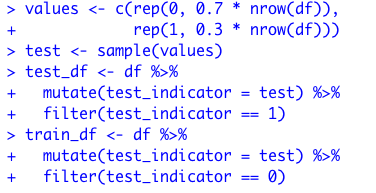
\includegraphics[scale=0.5]{traintest.png}
\end{figure}

\vspace{0.1cm}

We have now created two separate datasets, \texttt{test\_df} and \texttt{train\_df}, by randomly splitting our dataset into two groups, with 70\% of observations in the training dataset and 30\% in the testing dataset.

% break down what this is doing during class
\end{frame}

\begin{frame}{Training and testing data: in \texttt{R}}
We then use the training data to fit our model, and obtain predictions for the testing data:

\vspace{0.3cm}

\texttt{mod <- lm(data = train\_df, ...)} \\
\texttt{predictions <- predict(mod, newdata = test\_df)}

\vspace{0.3cm} \pause

It might also be useful to create a new object containing the observed outcomes for individuals in the testing data:

\vspace{0.3cm}

\texttt{observations <- test\_df \%>\% pull(outcome variable)}

\end{frame}

\begin{frame}{Training and testing data: Example in \texttt{R}}
Suppose we are (again) interested in predicting a baby's birthweight based on birth parent's age, marital status, whether or not they smoke during pregnancy, and weight prior to pregnancy. We first divide our data into training and testing data, fit the model on the training data, and then predict the outcomes for the testing data:

\begin{figure}
	\centering 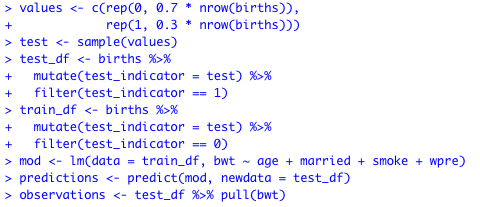
\includegraphics[scale=0.5]{traintest2.png}
\end{figure}
\end{frame}

\begin{frame}{Training and testing data: Example in \texttt{R}}
We now have predictions and observed outcomes for individuals in out testing dataset. For quantitative outcomes, a simple way to visualize how good our predictions are is with a scatterplot comparing the two.

\vspace{0.3cm}

\centering 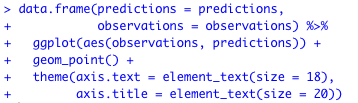
\includegraphics[scale=0.4]{predict_vs_obs_code.png} \vspace{0.1cm}

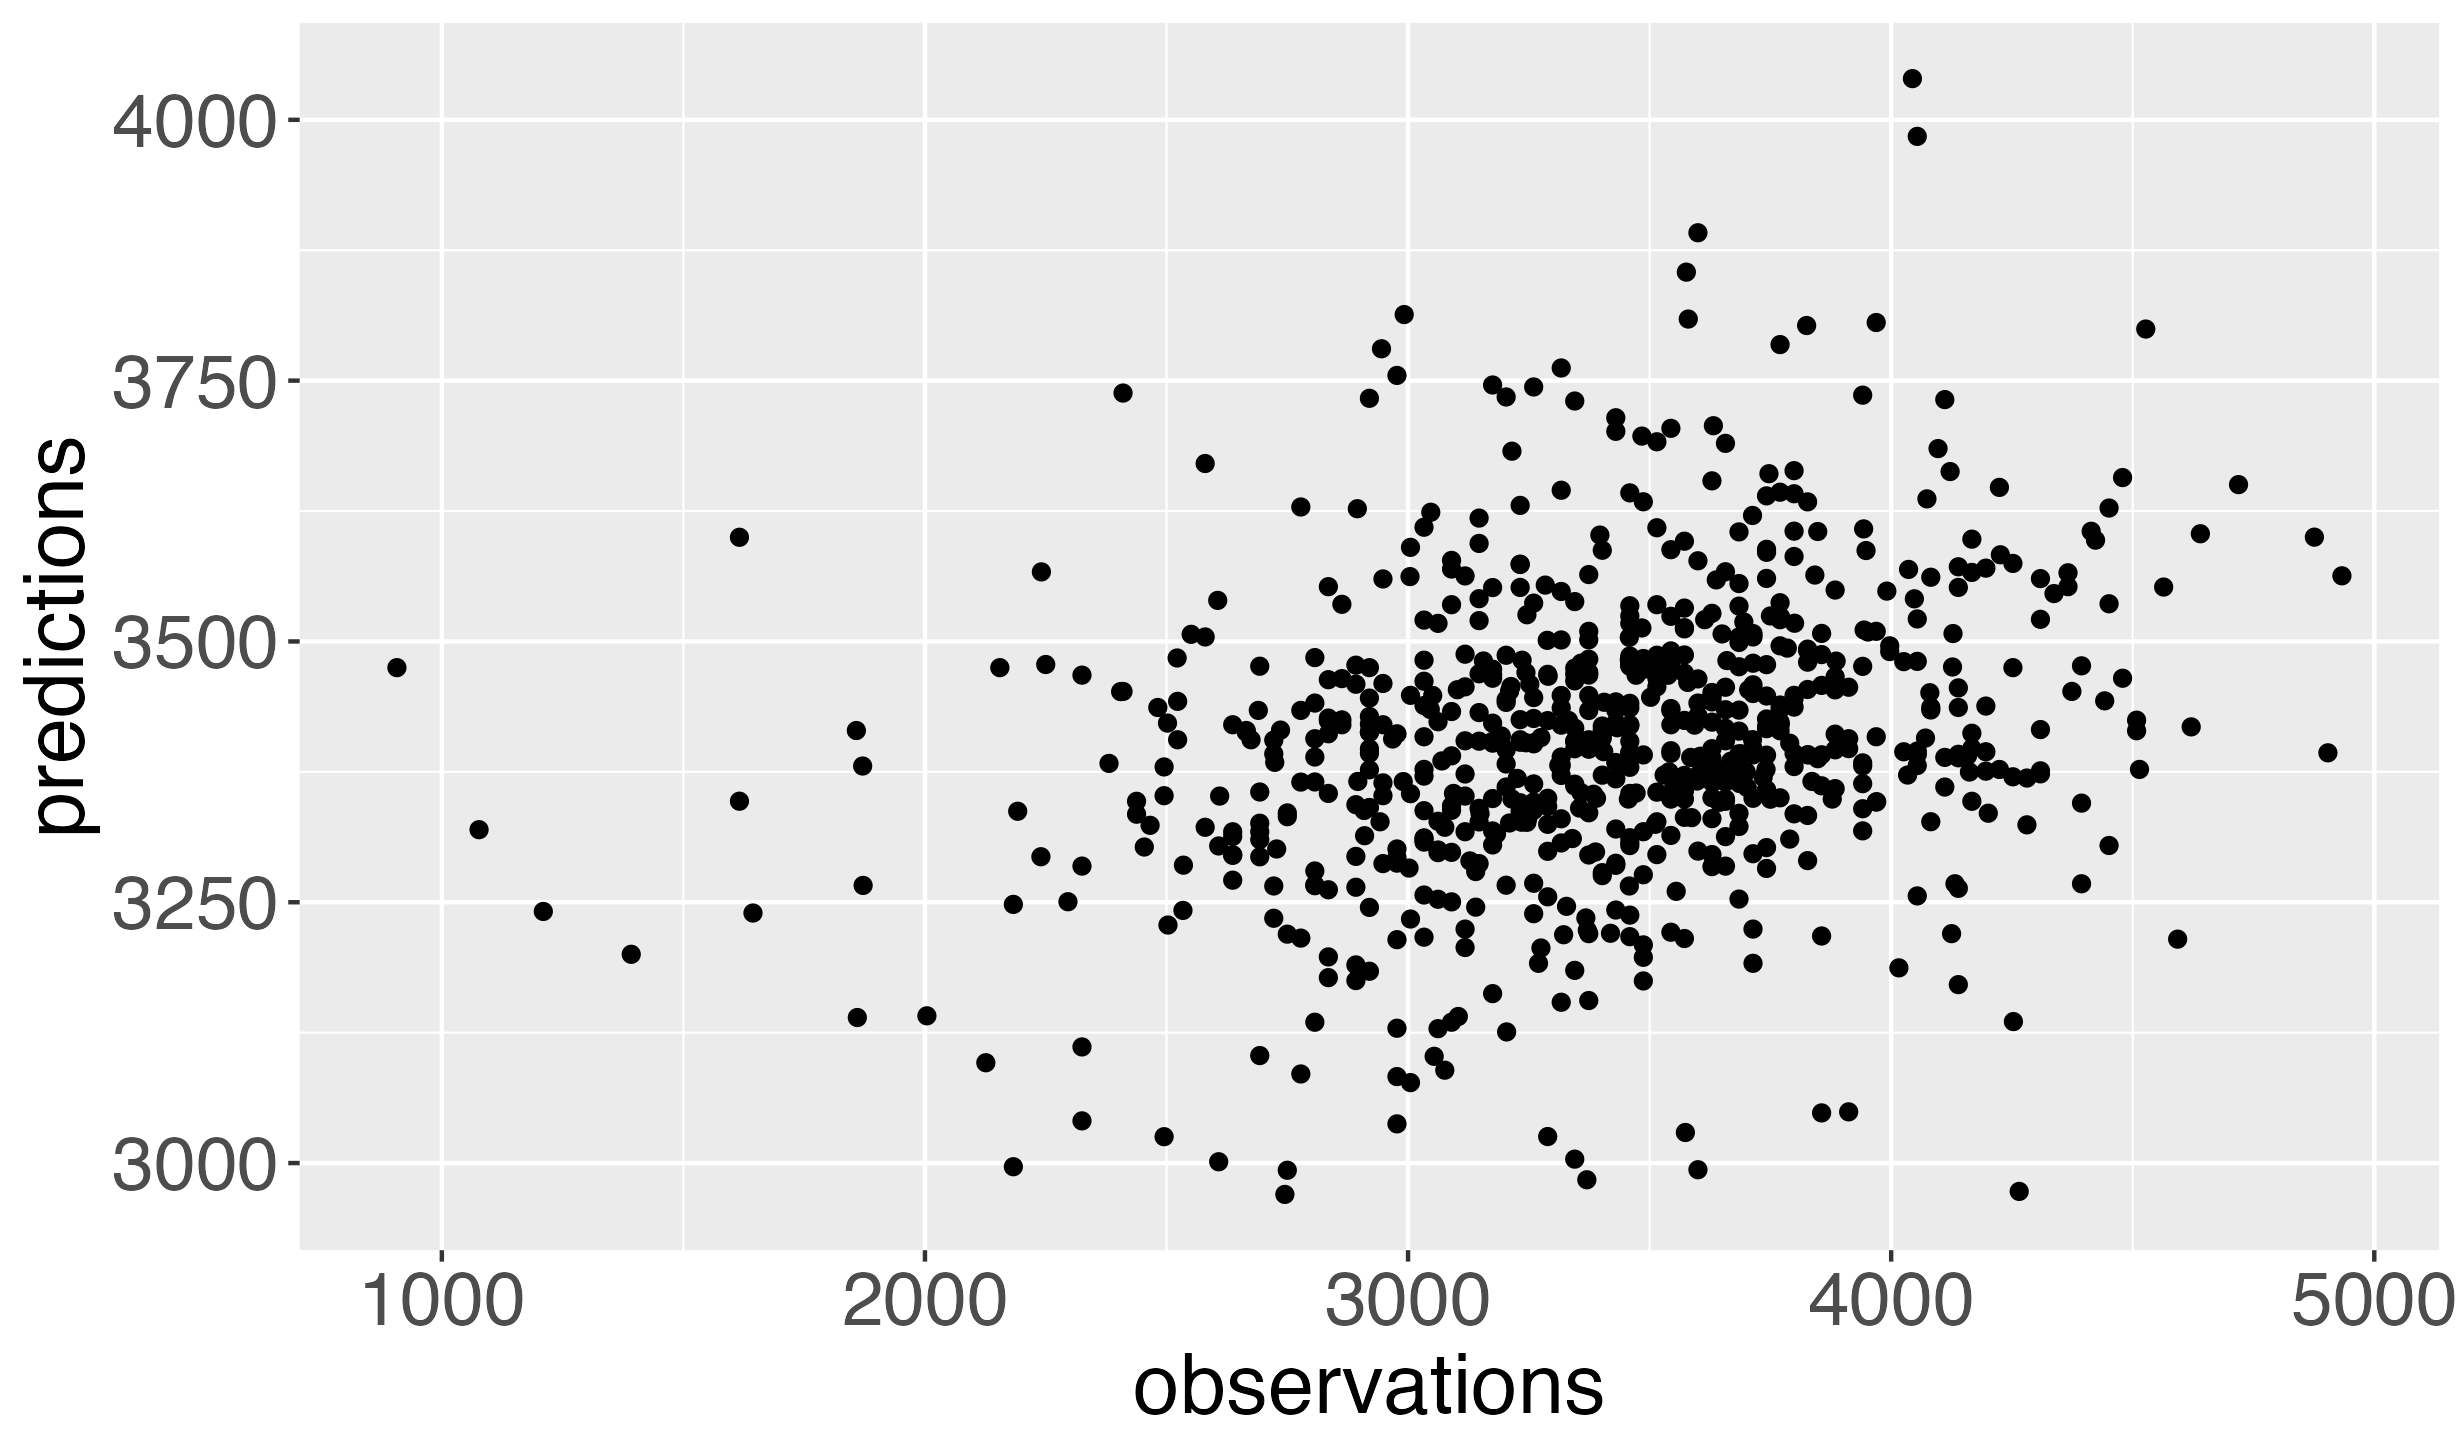
\includegraphics[scale=0.3]{predict_vs_obs.png}

\end{frame}

\begin{frame}{Training and testing data: Example in \texttt{R}}
\begin{figure}
	\centering 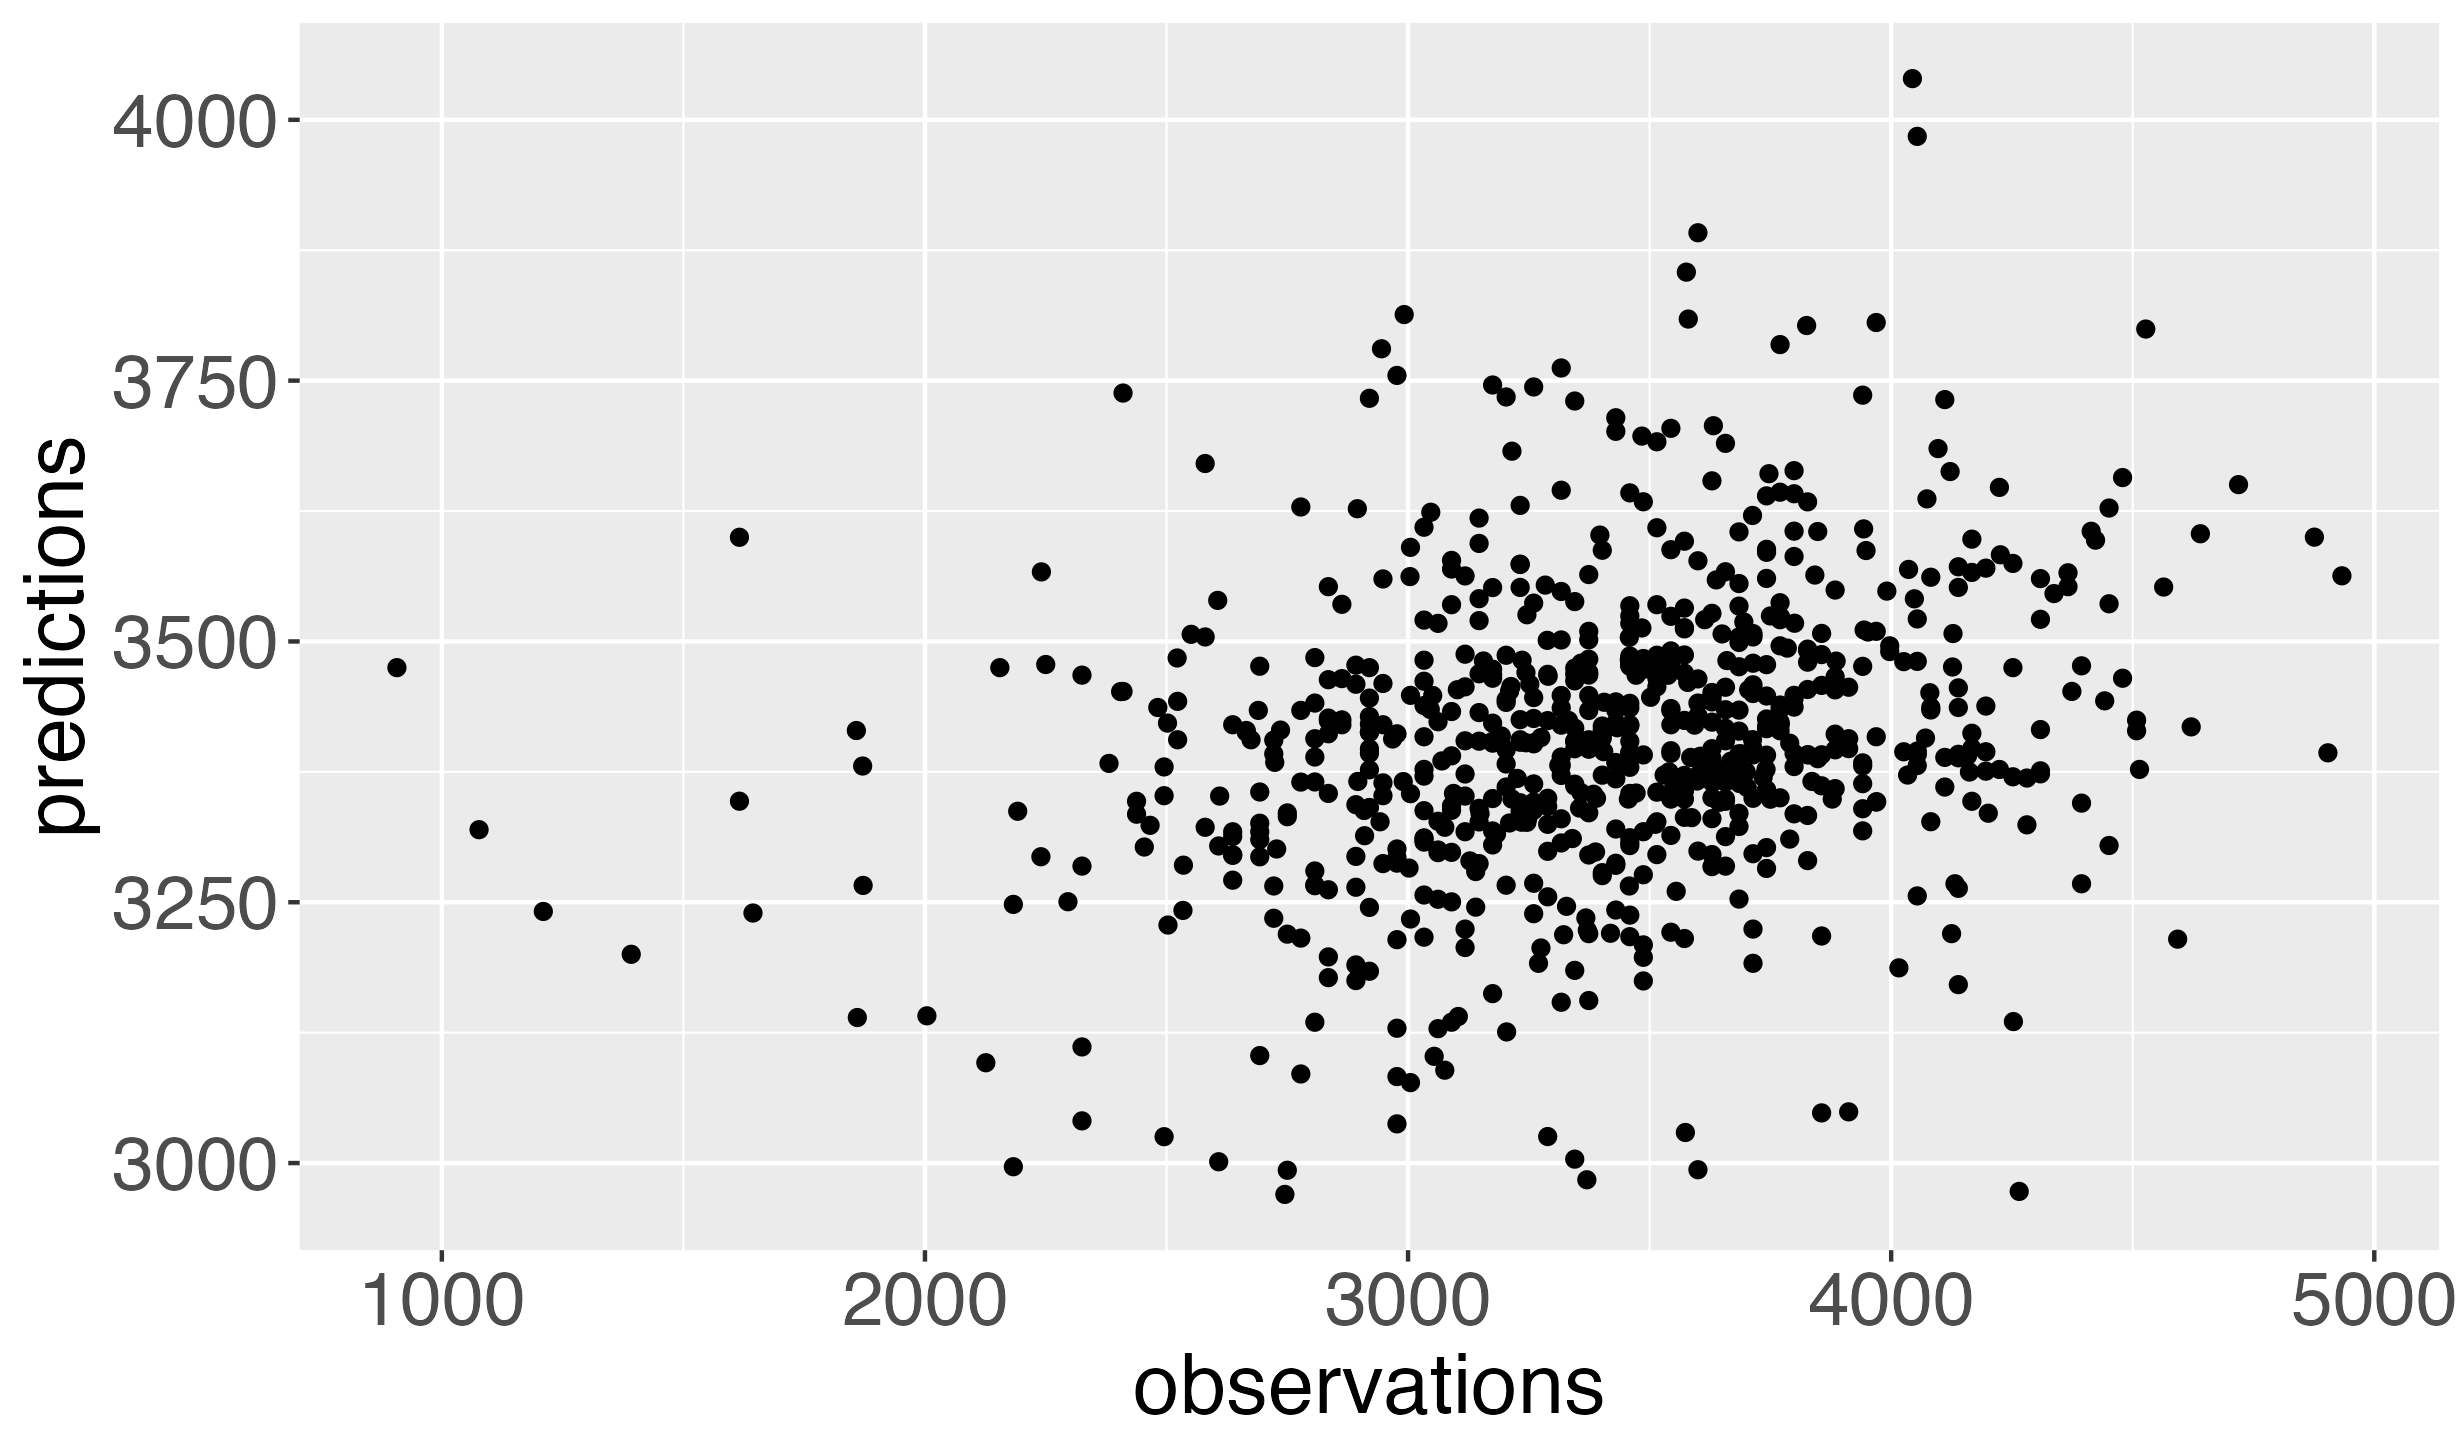
\includegraphics[scale=0.3]{predict_vs_obs.png}
\end{figure}

\textcolor{blue}{Question:} What would our scatterplot comparing observed outcomes and predictions look like if we were able to \textit{perfectly} predict the observed outcome? \pause

\vspace{0.3cm}

\textcolor{blue}{Answer:} If we perfectly predicted the observed outcome, we would have predictions = observations (which corresponds to the line $y = x$). All of our points would lie on the line $y = x$ in our scatterplot!

\end{frame}

\begin{frame}{Training and testing data: Example in \texttt{R}}
We can overlay a line with slope equal to 1 and intercept 0 on our scatterplot to see how well the points fall on the line, using the \texttt{geom\_abline} function:

\vspace{0.3cm}

\centering 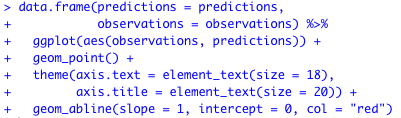
\includegraphics[scale=0.4]{predict_vs_obs_code2.png} \vspace{0.1cm}



\end{frame}

\begin{frame}{Training and testing data: Example in \texttt{R}}
\begin{figure}
	\centering 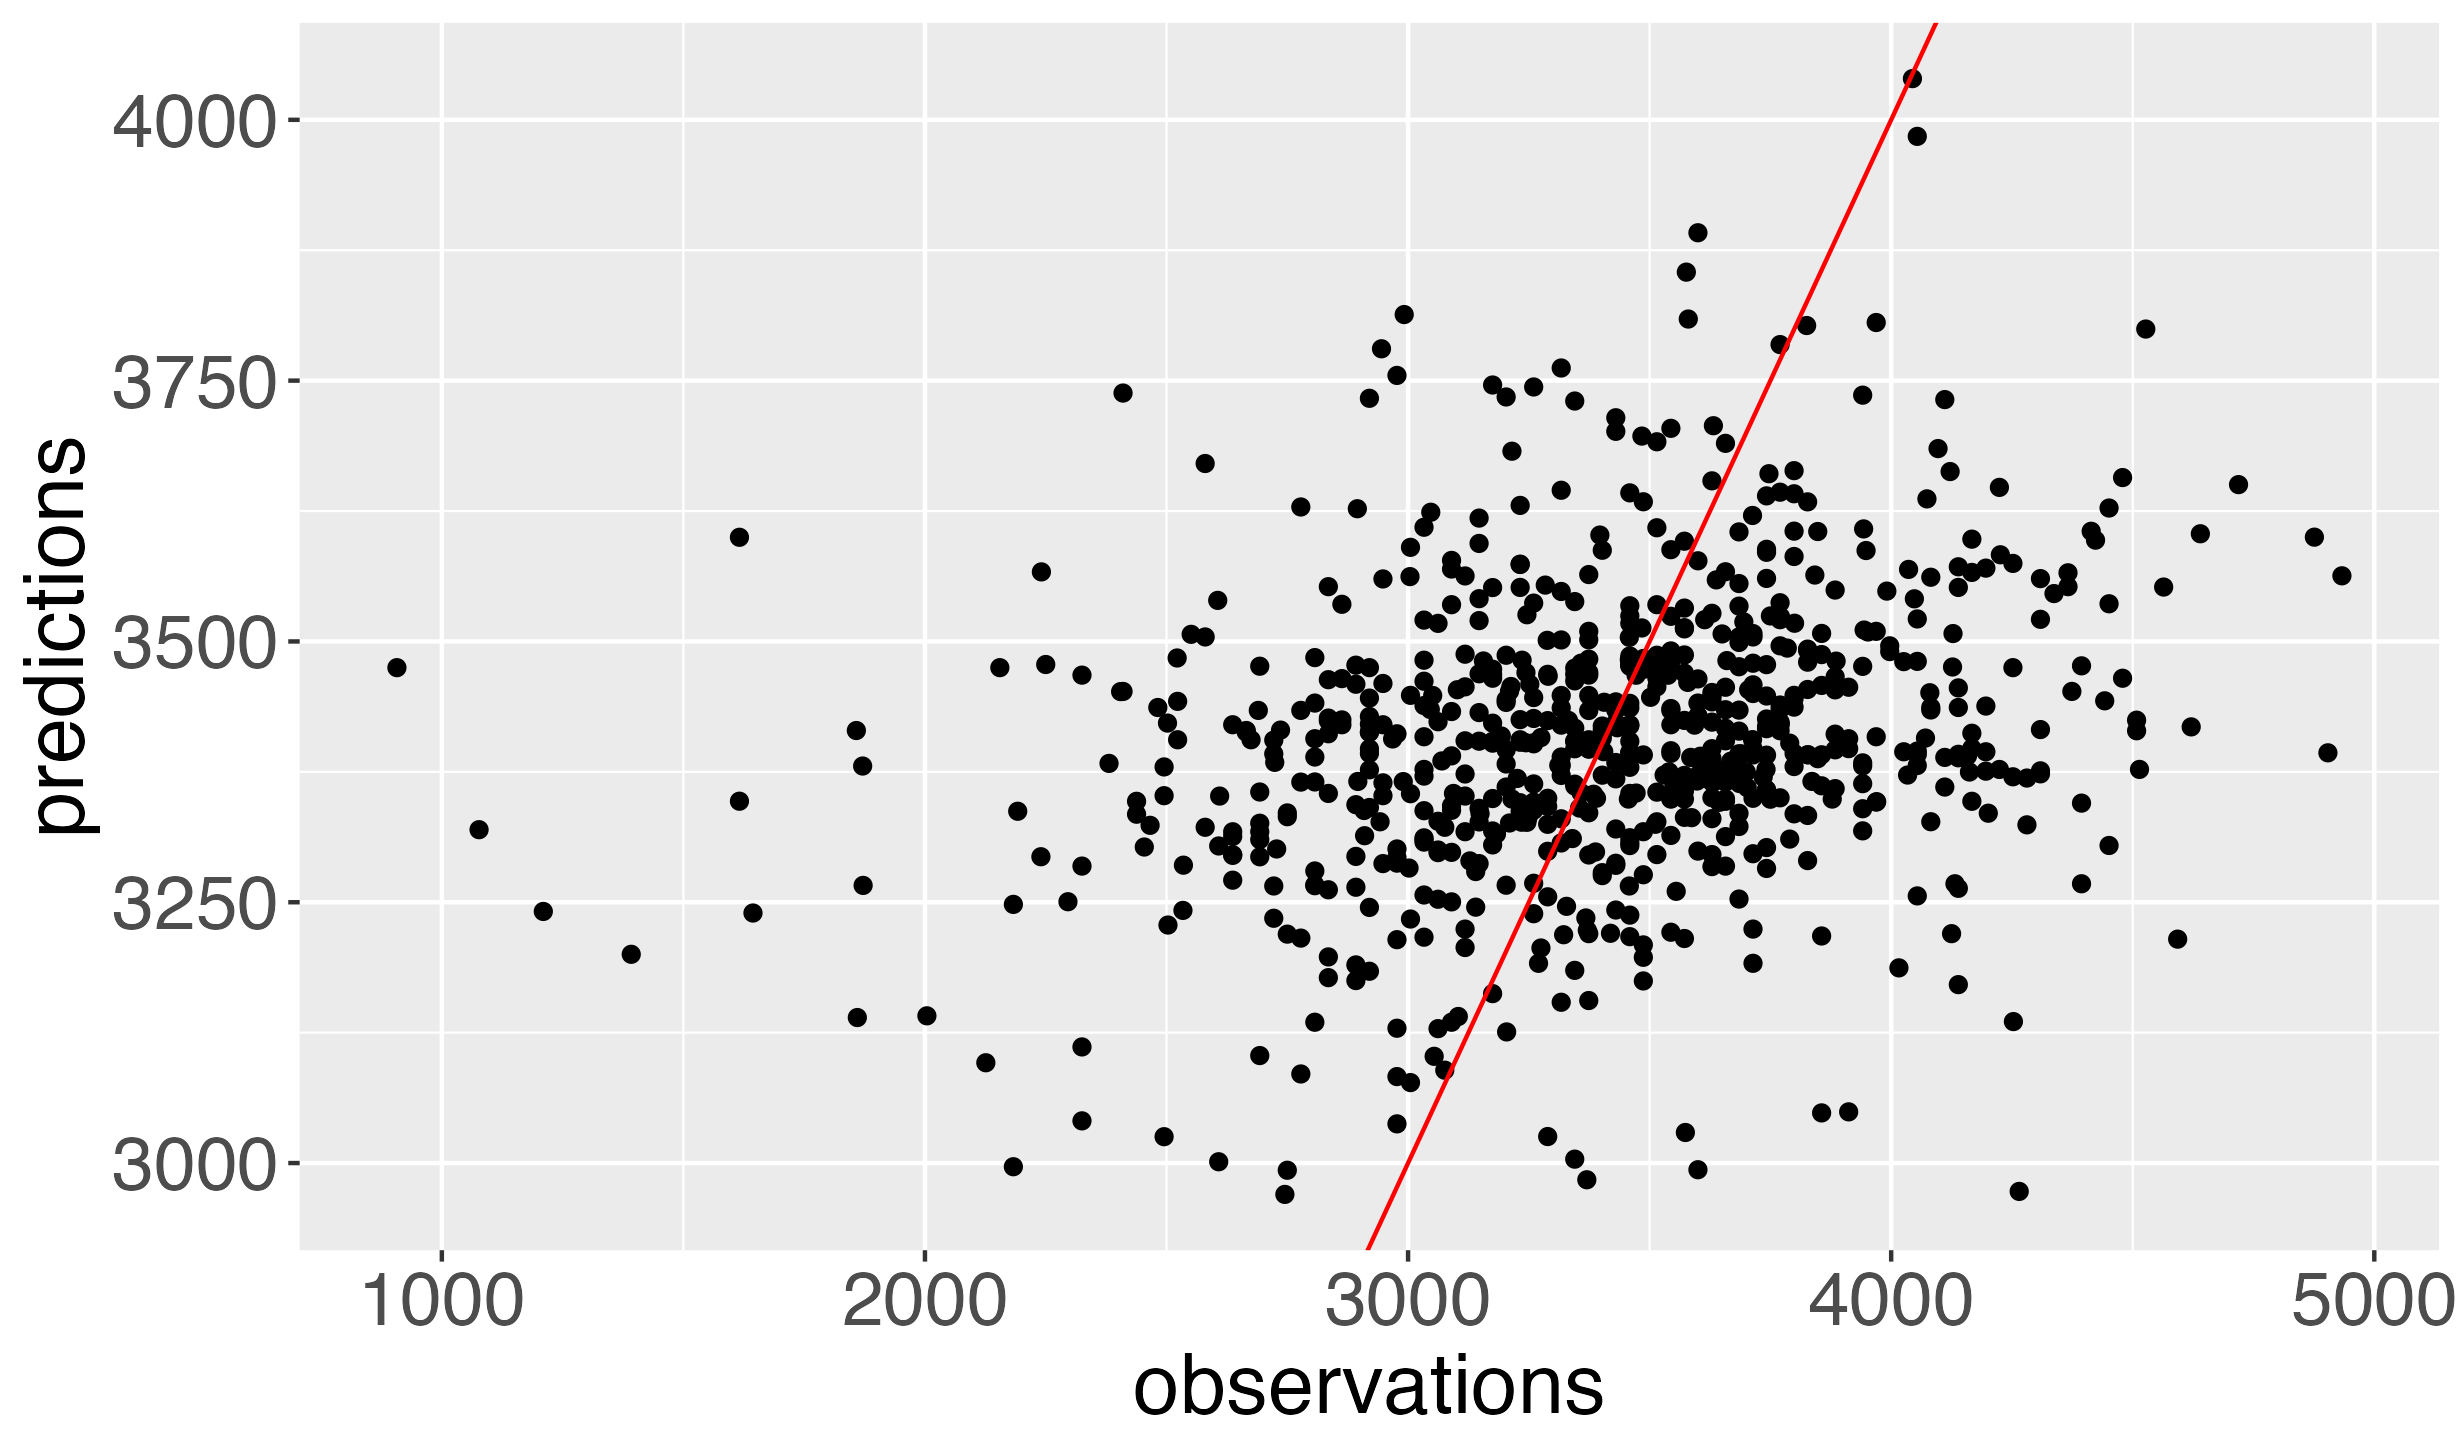
\includegraphics[scale=0.3]{predict_vs_obs2.png}
\end{figure}

Our predictions don't seem to be very good based on our scatter plot (the points in our graph do not fall on the line with slope equal to 1 and intercept 0). This is \textcolor{orange}{qualitative} way to assess how accurate our predictive model is.

\vspace{0.3cm}

We will now turn to \textcolor{orange}{quantitative} ways to assess prediction accuracy.
\end{frame}

% slide on why we care about model fit on testing data, not training data

\section{Measures of prediction accuracy}

\subsection{$R^2$}


\begin{frame}{$R^2$: Coefficient of determination}
One way to assess how good our predictions are is to determine the proportion of the variance in the outcome explained by the covariates in our predictive model.

\vspace{0.3cm}

\textcolor{blue}{$R^2$ (also called the Coefficient of determination)}: the proportion of the variance in the outcome explained by the covariates in the model. 

\vspace{0.3cm}

If $R^2$ can take values between 0 and 1:

\vspace{0.3cm}

\begin{itemize}
	\item If $R^2$ is close to 0, then the covariates in our predictive model does not do a good job of explaining the variation in the observed outcome
	\item If $R^2$ is close to 1, then the covariates in our predictive model do a good job of explaining the variation in the observed outcome
\end{itemize}

\vspace{0.3cm}

$R^2$ is a metric that is computed on a \textit{training} dataset, or a full dataset, and is often used for \textcolor{blue}{model comparison}, where we have a set of possible predictive models and are trying to determine which is best.
\end{frame}

\begin{frame}{$R^2$: Multiple vs. Adjusted}
$R^2$ can be found in regression output from the \texttt{lm} function. The output gives us two types of $R^2$:

\vspace{0.3cm}

\begin{itemize}
	\item \textcolor{blue}{Multiple $R^2$}: $$1 - \frac{\sum_{i = 1}^n (Y_i - \hat{Y}_i)^2}{\sum_{i = 1}^n (Y_i - \bar{Y}_i)^2} \hspace{0.3cm} 
\includegraphics[scale=0.01]{chilipepper.png}$$  [1 - (sum of squared residuals / total sum of squares)] 
	\item \textcolor{blue}{Adjusted $R^2$}: Similar to $R^2$, but accounts for the number of covariates in the model
\end{itemize}

\end{frame}

\begin{frame}{$R^2$: Multiple vs. Adjusted}
Key information:

\vspace{0.3cm}

\begin{itemize}
	\item Multiple $R^2$ will \textit{always} increase from adding additional covariates into a model
	\item Adjusted $R^2$ will not necessarily increase from adding additional covariates into a model, because it penalizes adding additional variables into your model that don't improve prediction very much
	\item Adjusted $R^2$ does not have the same interpretation as $R^2$ (its interpretation is less straightforward)
\end{itemize}

\end{frame}

\begin{frame}{$R^2$: Multiple vs. Adjusted}

\textcolor{blue}{Question:} Suppose we are choosing between two predictive models, and determining which is better based on $R^2$. A higher $R^2$ means a higher proportion of variation in the outcome is being explained by the covariates in the model, so we're inclined to choose the model with higher $R^2$. Why might we prefer adjusted $R^2$ to multiple $R^2$? \pause

\vspace{0.3cm}

\textcolor{blue}{Answer:} Since multiple $R^2$ increases from adding additional covariates into a model, we would always be inclined to choose the model with the most covariates. This could lead us to choose a model that is \textcolor{orange}{overfit} to our data.

\end{frame}

\begin{frame}{Overfitting}

Overfitting occurs when we fit a statistical model that corresponds too exactly to our observed data (often our training dataset), which tends to lead to worse predictions for new observations (often our testing dataset).

\vspace{0.3cm}

Overfitting can involve:

\vspace{0.3cm}

\begin{itemize}
	\item Including too many covariates in a model 
	\item \textcolor{blue}{Interpolation} (fitting a curve through each point exactly), or specifying another relationship between covariates and the outcome that is ``overfit" to the observed data
\end{itemize}

\end{frame}

\begin{frame}{Overfitting: Example}
Suppose we collect data for an outcome $Y$ and predictor $X$. We visualize our data in the scatter plot below:

\vspace{0.3cm}

\centering 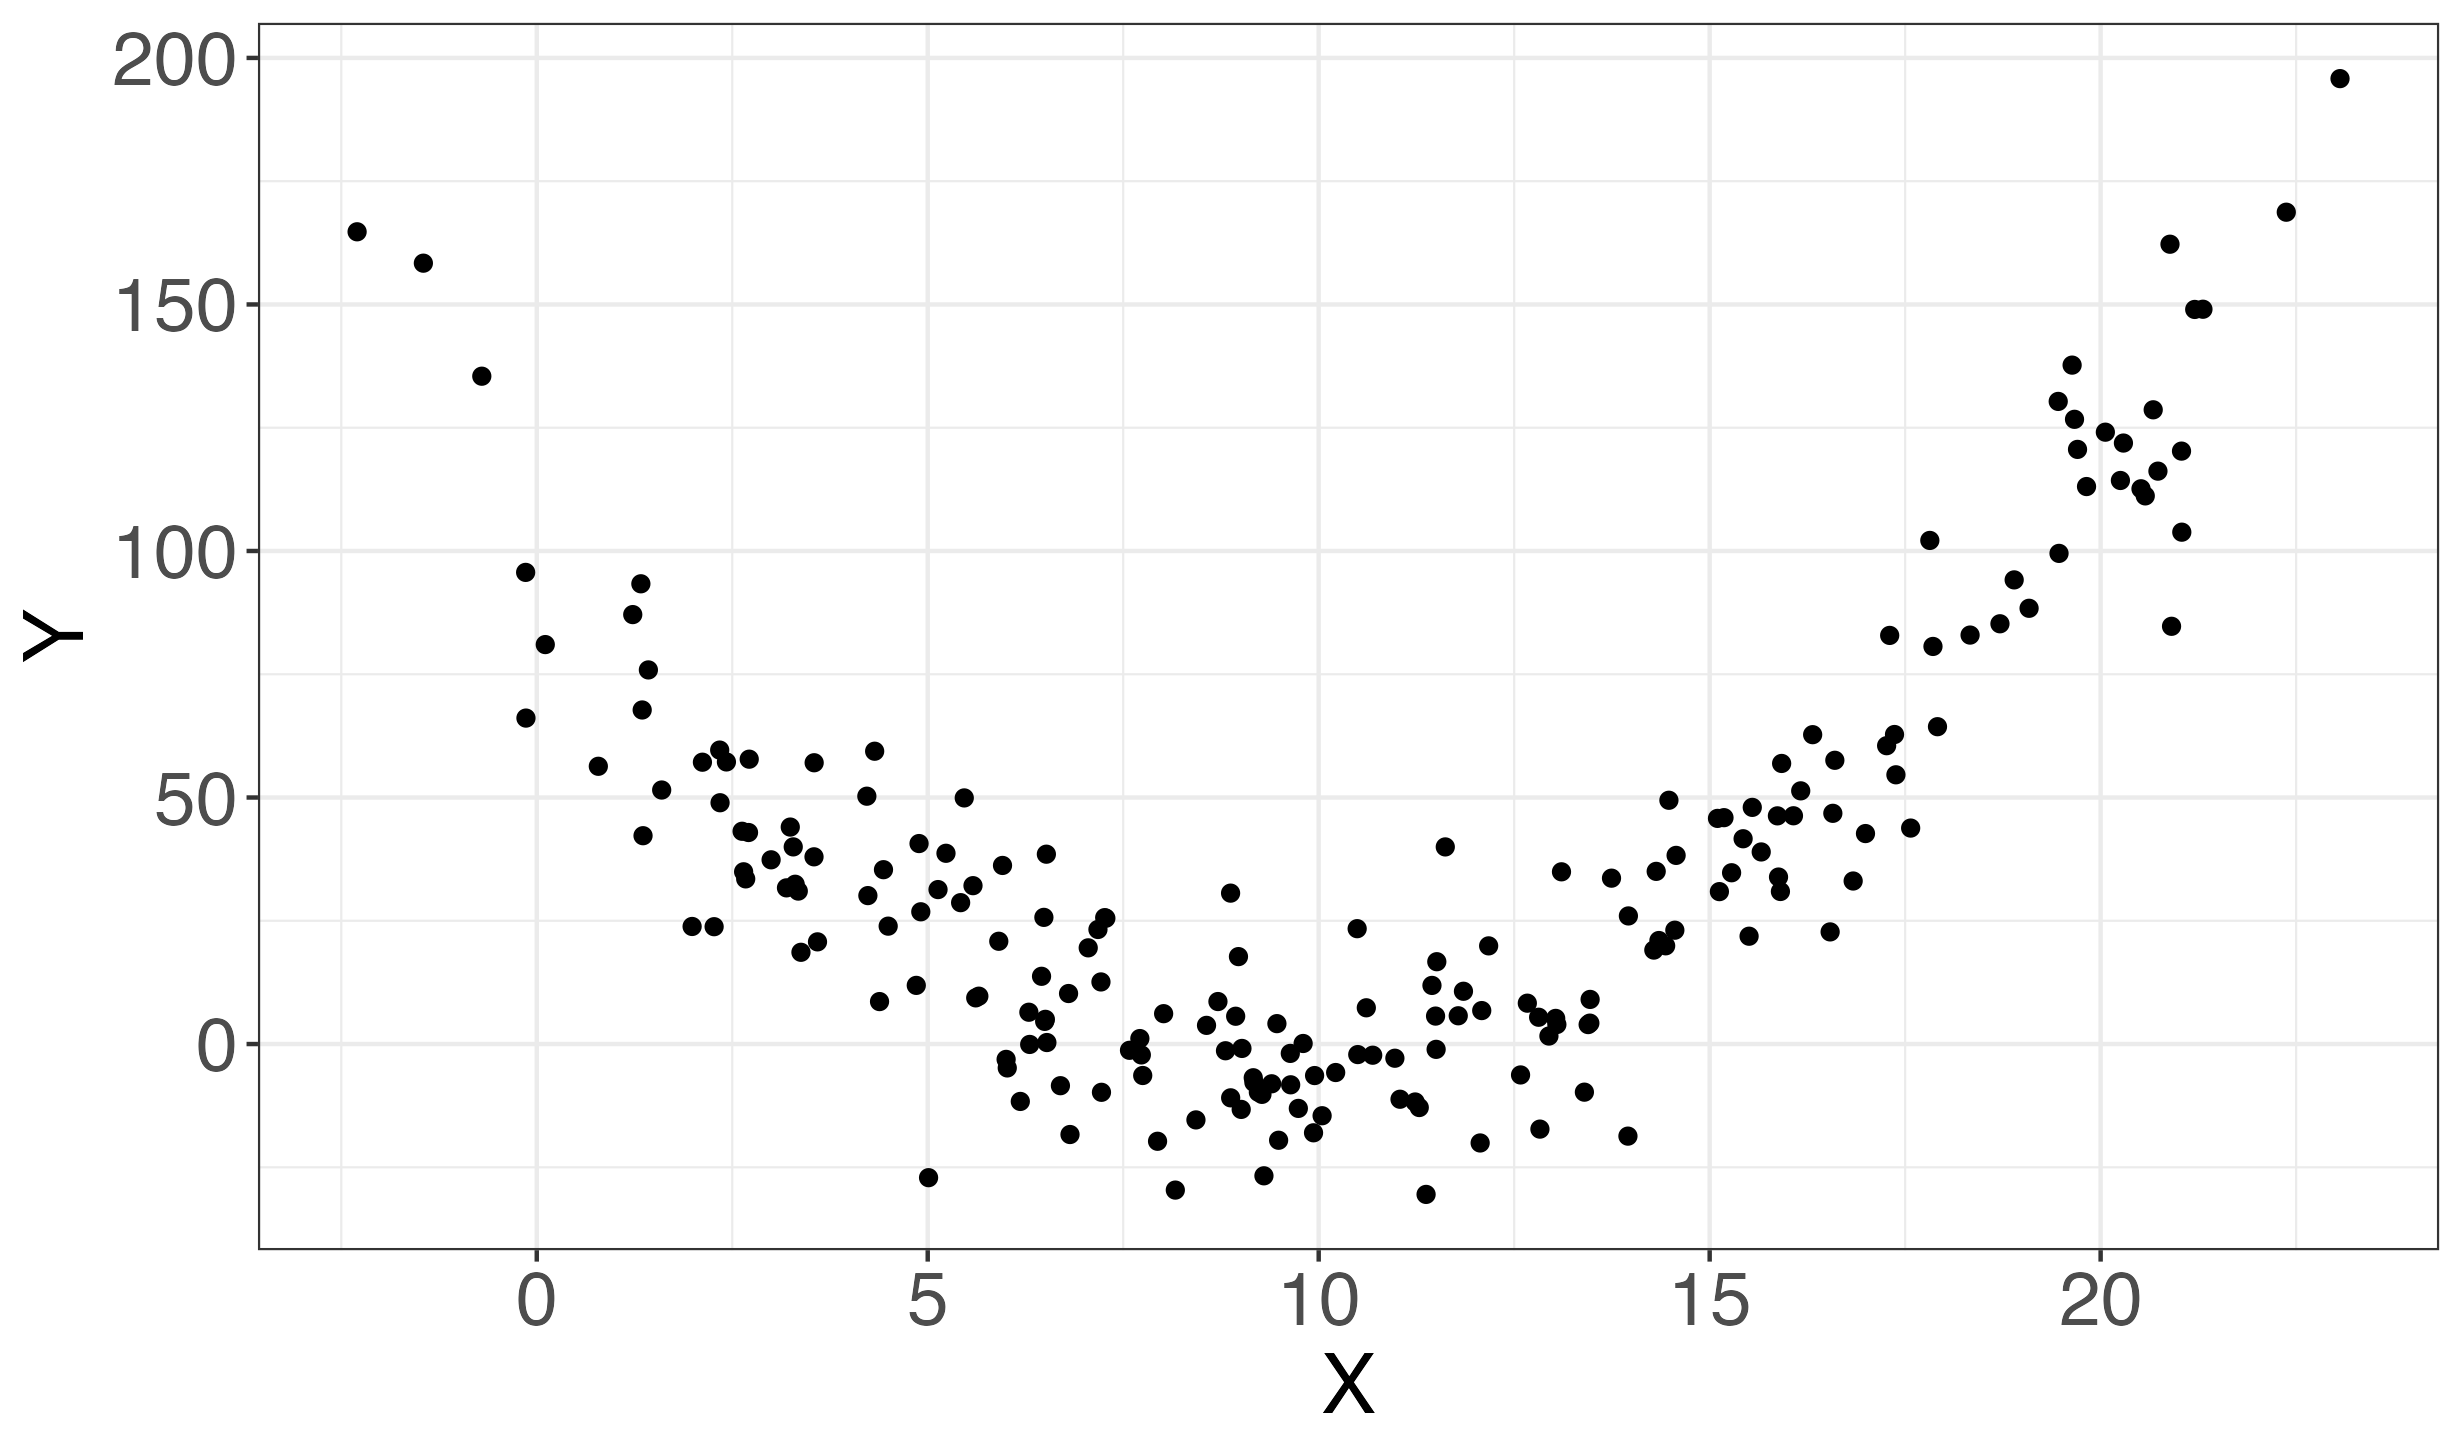
\includegraphics[scale=0.4]{overfit1.png}
\end{frame}

\begin{frame}{Overfitting: Example}
We could fit a simple linear regression model to our data, but this likely wouldn't produce great predictions\dots

\vspace{0.3cm}

\centering 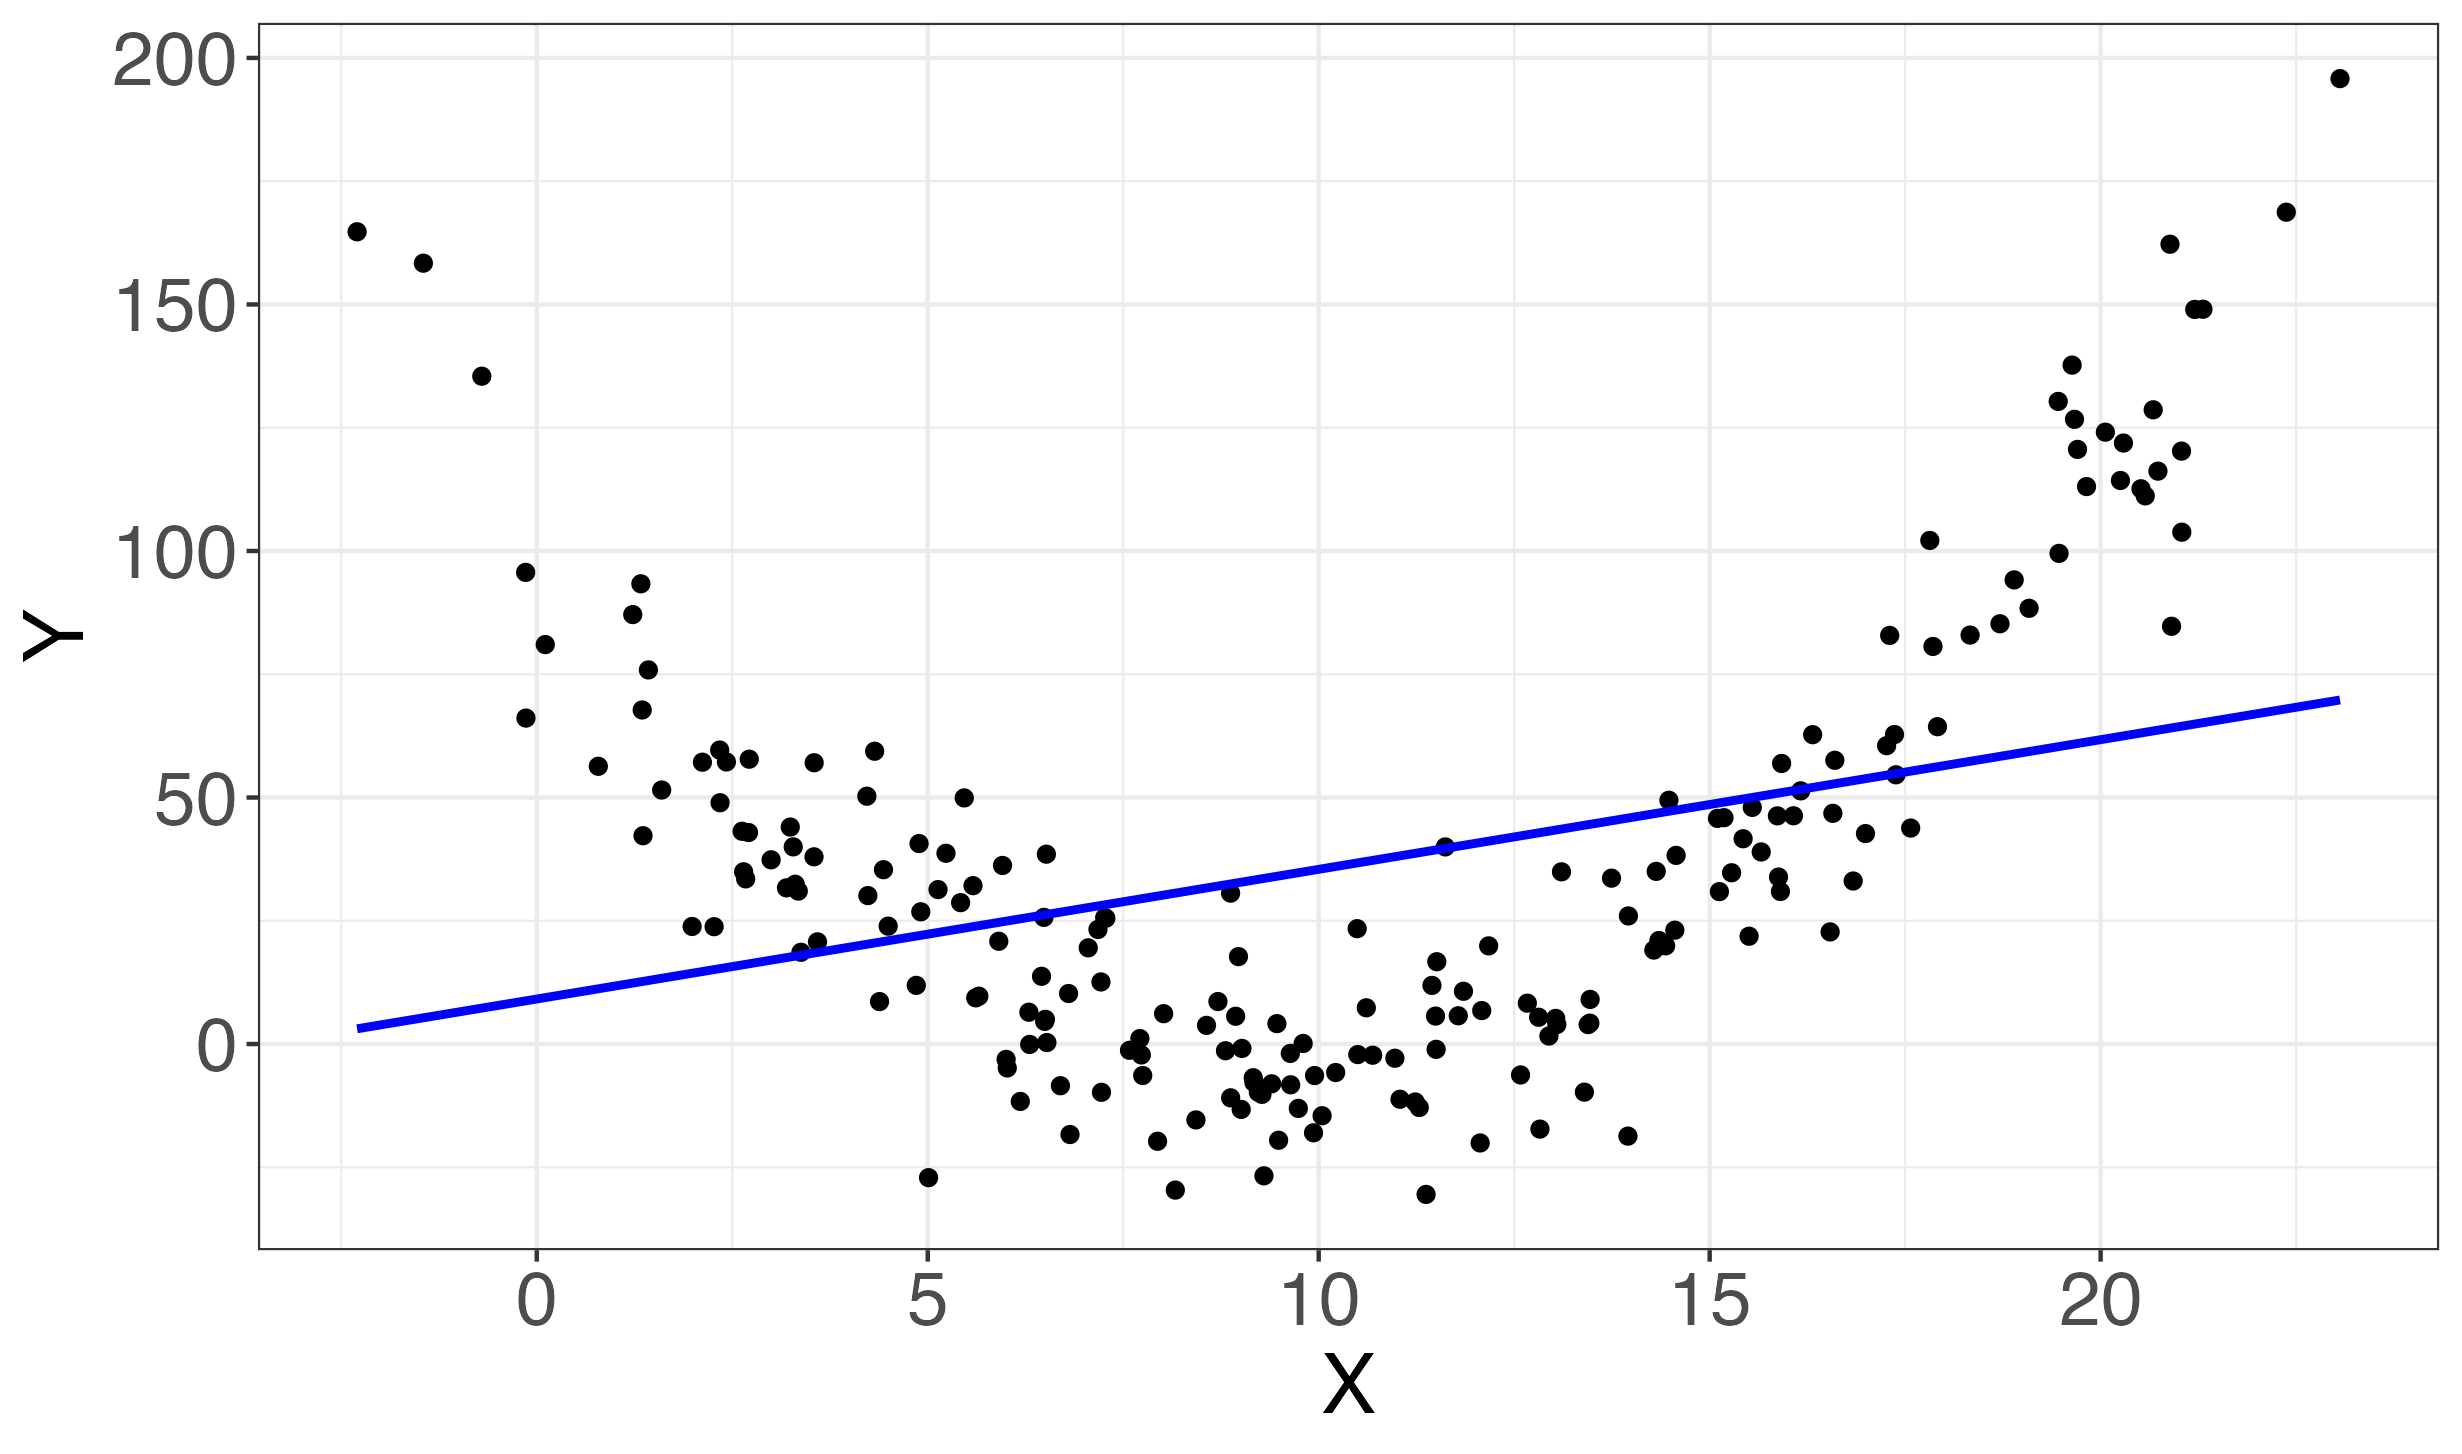
\includegraphics[scale=0.4]{overfit2.png}
\end{frame}

\begin{frame}{Overfitting: Example}
We could add an additional covariate term to our model, namely $X^2$\dots

\vspace{0.3cm}

\centering 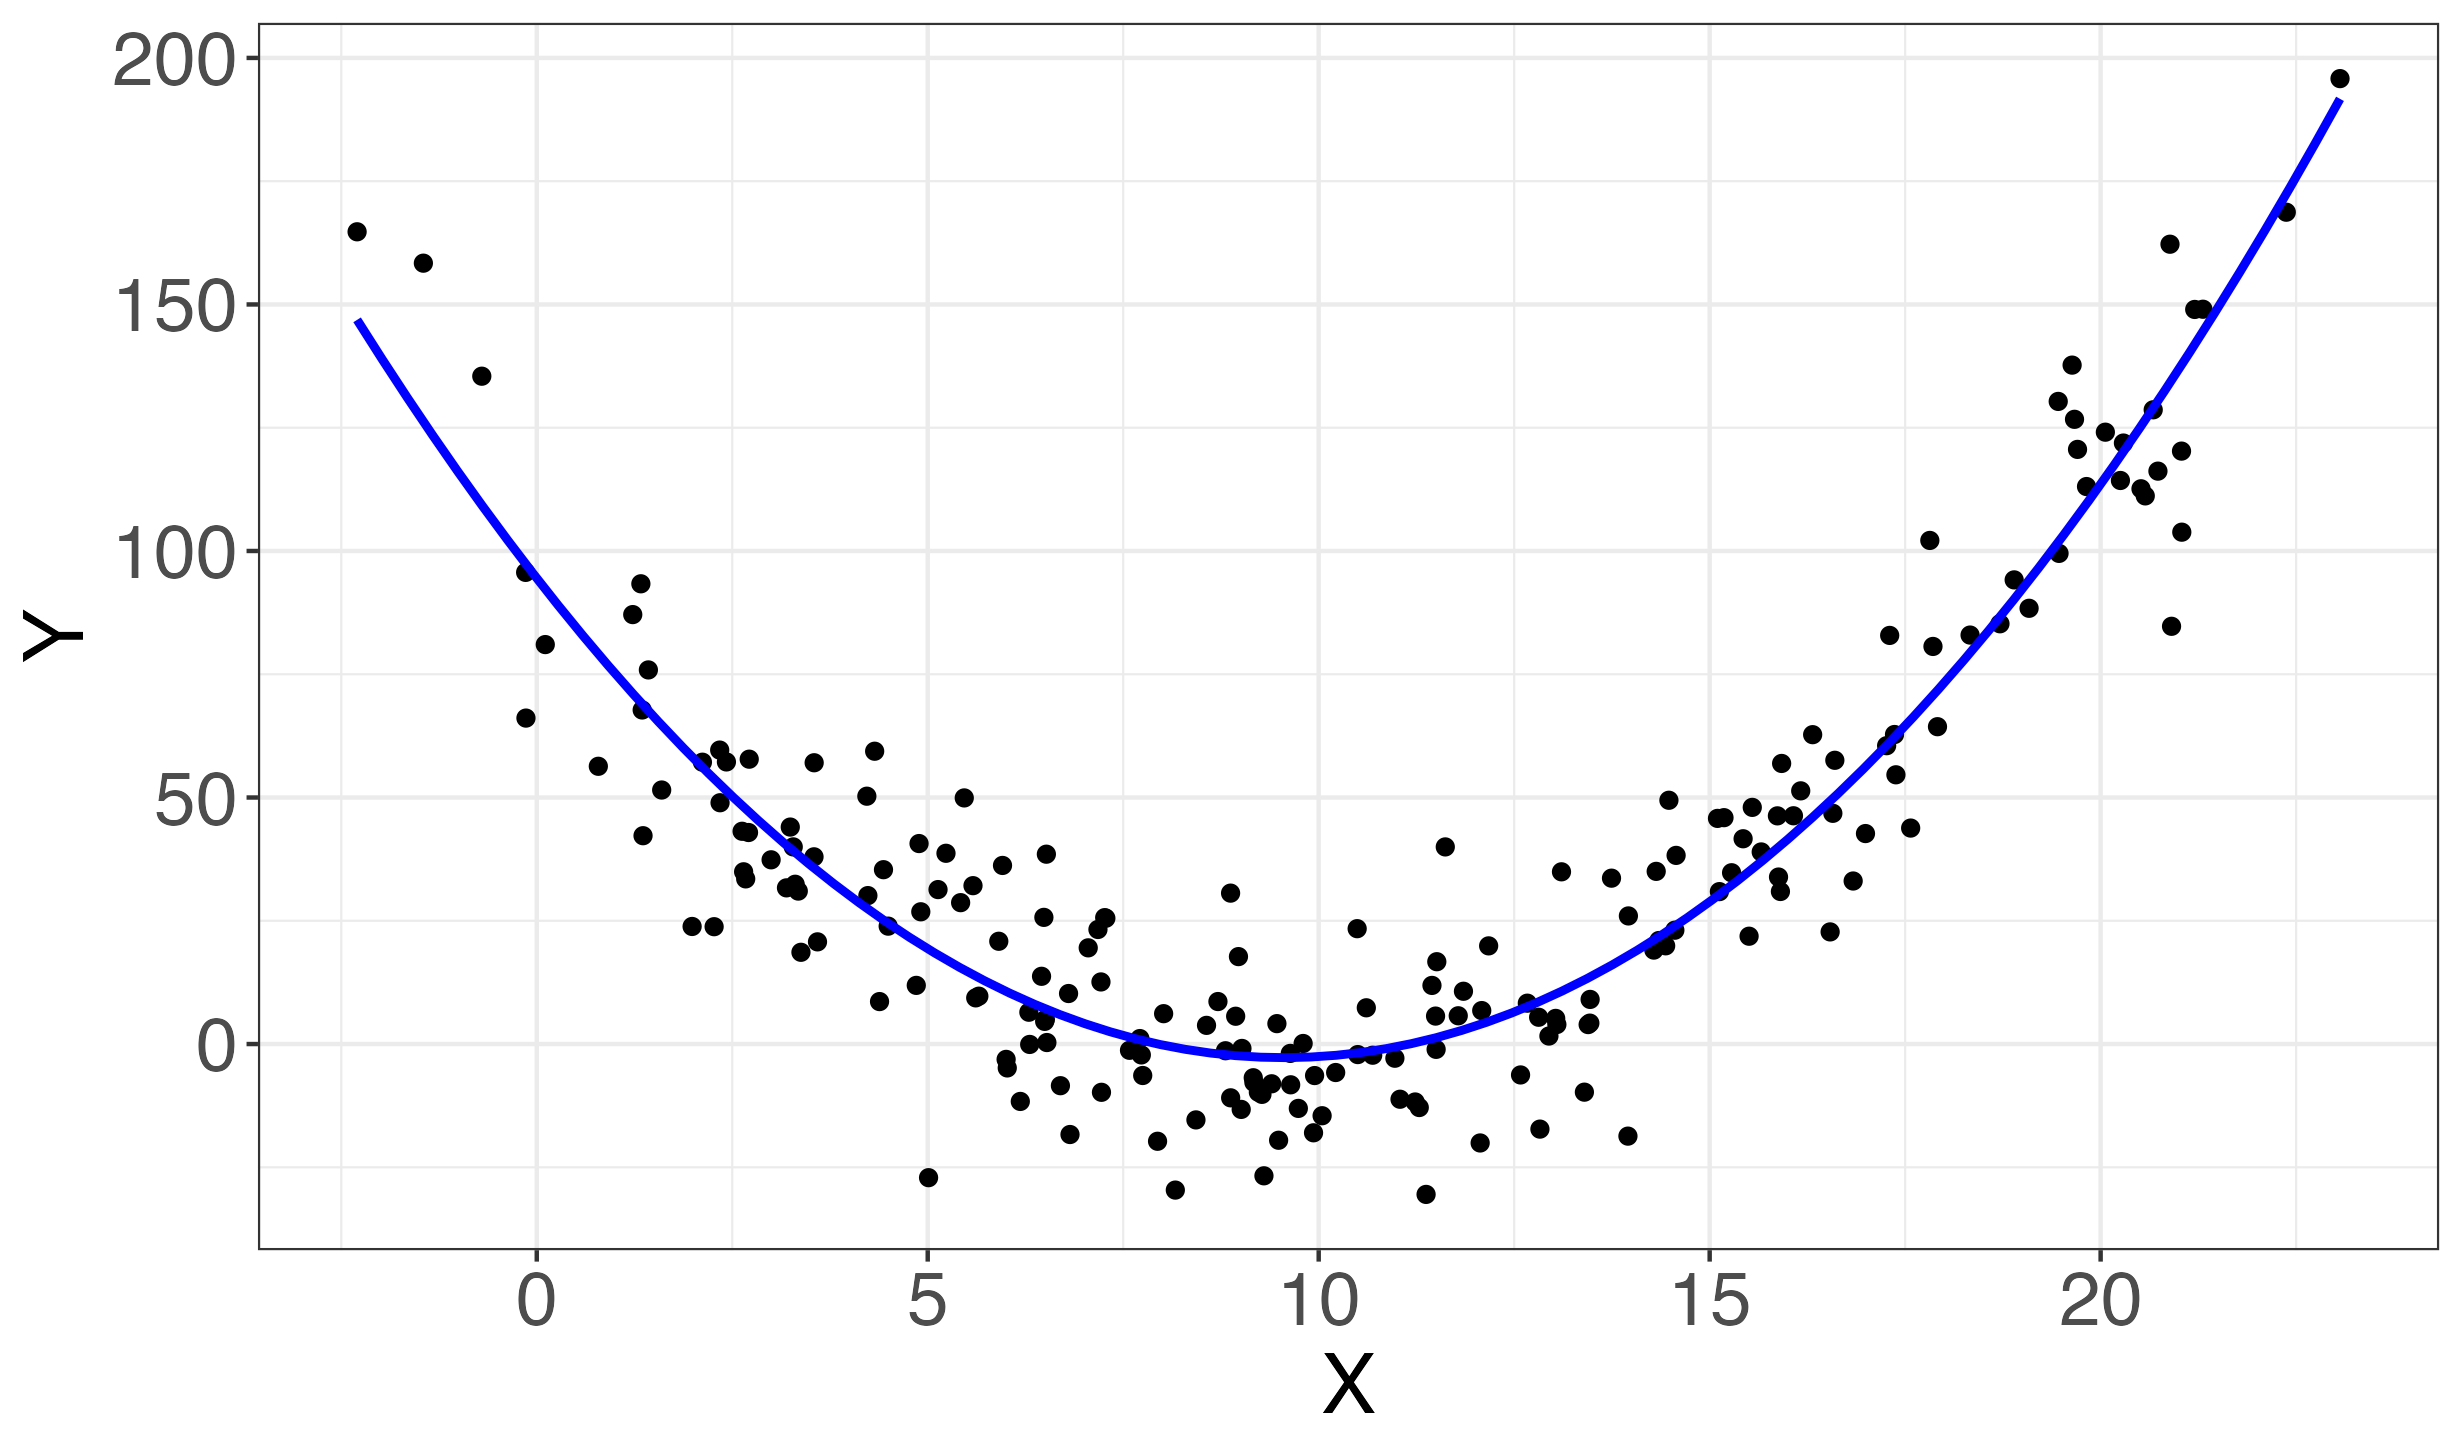
\includegraphics[scale=0.4]{overfit3.png}

\end{frame}

\begin{frame}{Overfitting: Example}
Or we could include \textit{many} additional covariate terms, for higher order polynomials (here, up to $X^{13}$)\dots

\vspace{0.3cm}

\centering 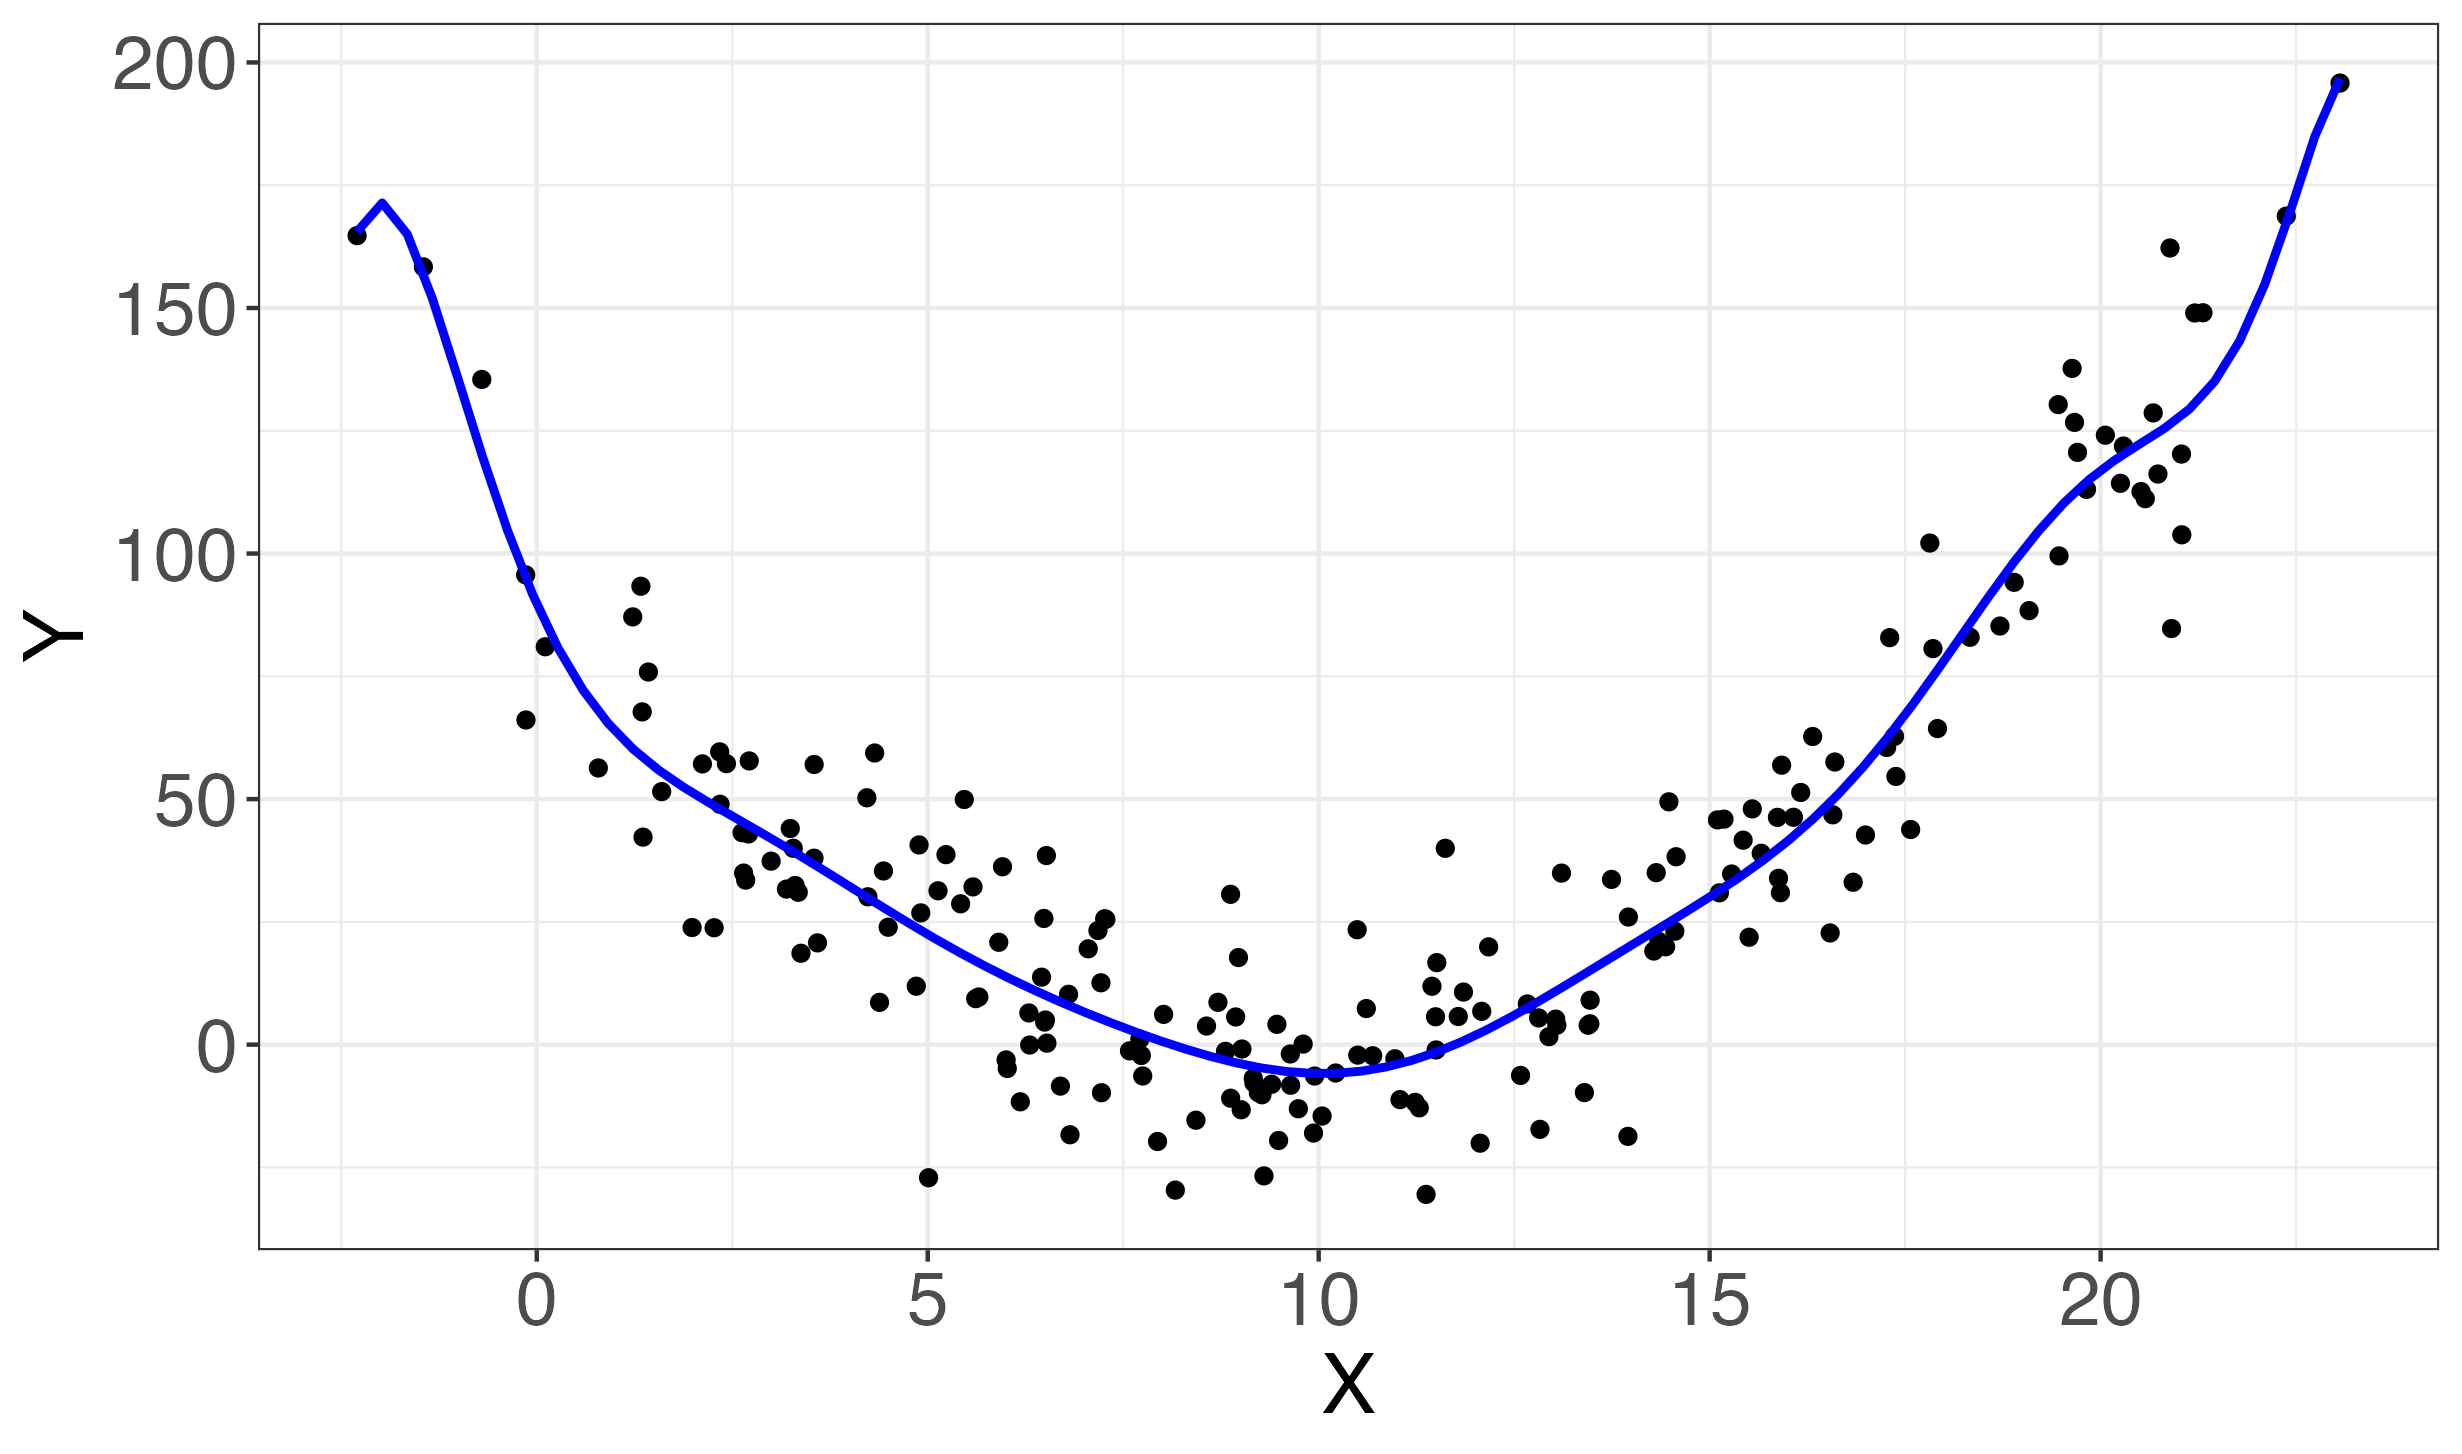
\includegraphics[scale=0.4]{overfit4.png}

\end{frame}

\begin{frame}{Overfitting: Example}
OR we could \textcolor{orange}{interpolate} to get perfect predictions for all of our observed data\dots

\vspace{0.3cm}

\centering 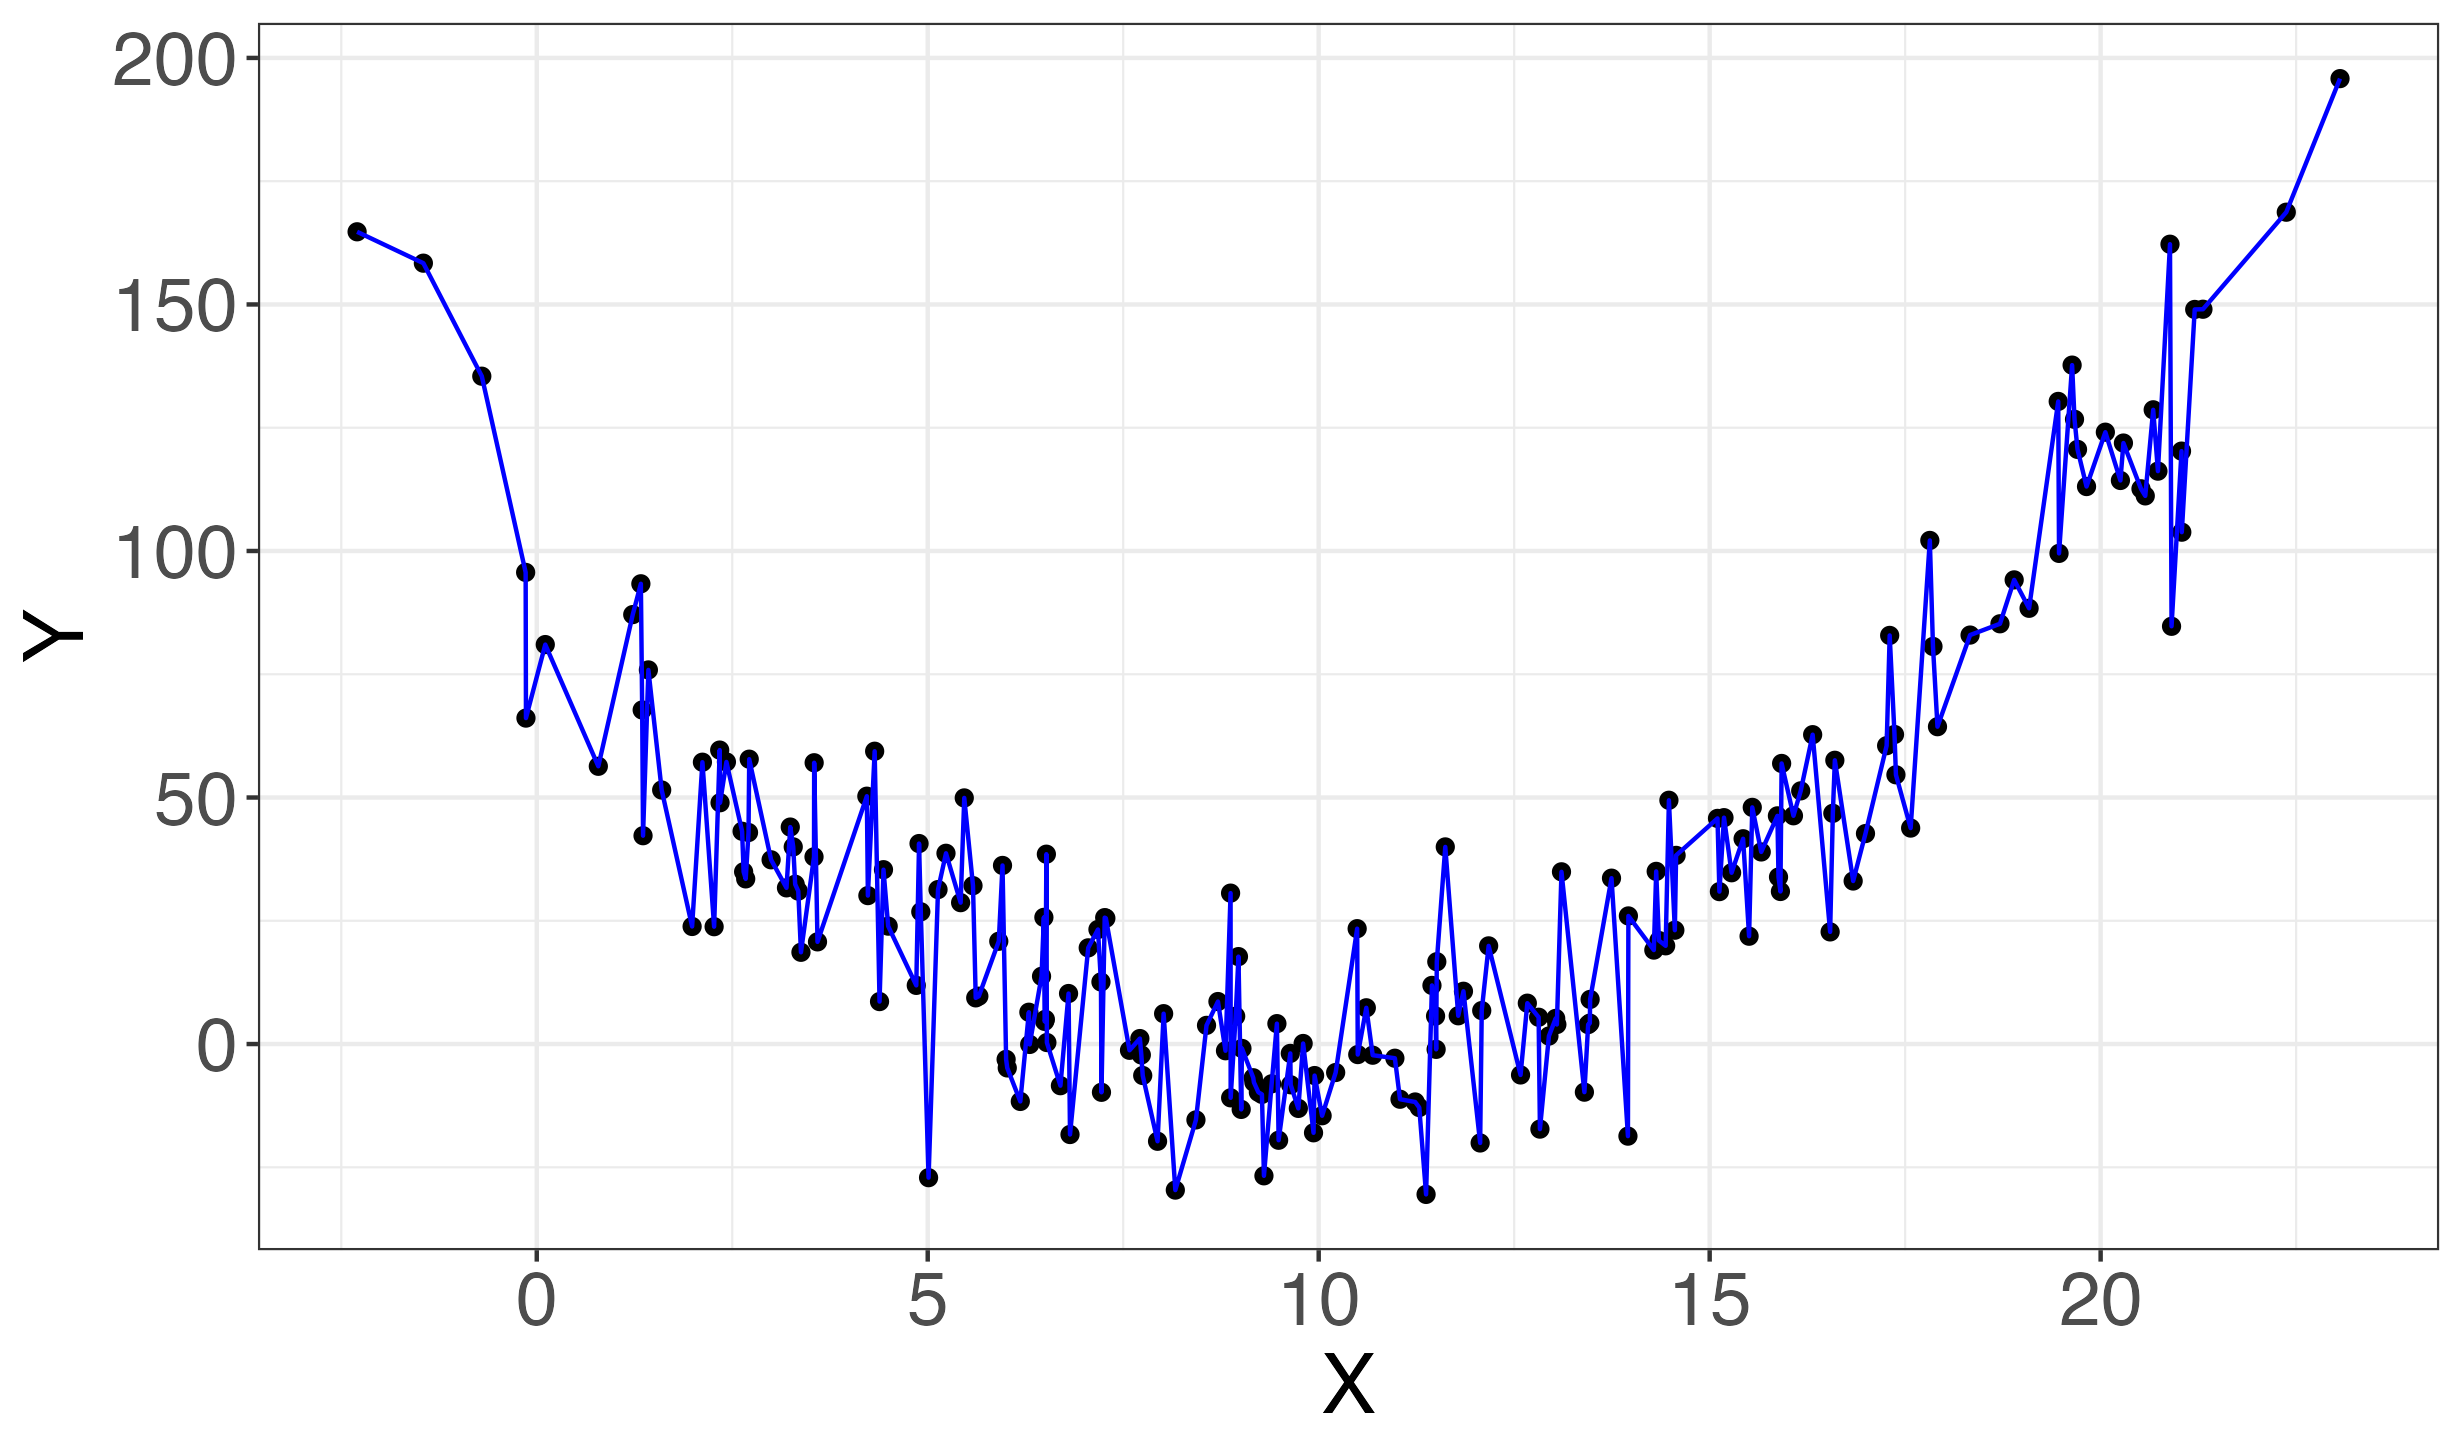
\includegraphics[scale=0.4]{overfit5.png}
\end{frame}

\begin{frame}{Overfitting Example}
For each of these cases (other than interpolation) and extending to additional polynomials, we can fit a linear regression model and get adjusted and multiple $R^2$ values.

\vspace{0.3cm}

\begin{table}
	\begin{tabular}{l|r|r}

Model & Mult. $R^2$ & Adj. $R^2$ \\
\hline
$Y \sim X$ & 0.121 & 0.117\\
\hline
$Y \sim X + X^2$ & 0.877 & 0.876\\
\hline
$Y \sim X + X^2 + \dots + X^{13}$ & 0.888 & 0.880 \\
\hline
\vdots & \vdots & \vdots \\
\hline
$Y \sim X + X^2 + \dots + X^{15}$ & 0.8897 & 0.8814 \\
\hline
$Y \sim X + X^2 + \dots + X^{15} + X^{16}$ & 0.8898 & 0.8808
\end{tabular}
\end{table}

\vspace{0.3cm} At a certain point, adjusted $R^2$ decreases with the inclusion of an additional covariate in the model (in this example, $X^16$), while multiple $R^2$ continues to increase.
	
\end{frame}

\begin{frame}{Overfitting: Why does it matter?}
In the previous example, the model with only two covariates ($X$ and $X^2$) is likely complex enough to give us good predictions for new observations. When we include too many covariates in our model, we run the risk of overfitting our model to the data, and making worse predictions down the line.

\vspace{0.3cm}

Remember that we care about how accurate our prediction model is at predicting \textit{new} observations (often our testing data). If we focus on choosing a predictive model solely based on $R^2$ (either multiple or adjusted) from fitting our model to training data, we may be tempted to choose a model that predicts the training data outcome very well but fails for new observations.

\vspace{0.3cm}

\textcolor{orange}{Rule of thumb:} If two models differing by a single covariate have $R^2$ values that are very similar (within 0.01 of each other), it is reasonable to choose the model with fewer covariates, for the purposes of this course. \small (\textit{However}, there are additional prediction accuracy metrics we can consider in addition to $R^2$ that may supplement your model choice decision, which we'll talk about after an example)
\end{frame}

\begin{frame}{$R^2$: Example in \texttt{R}}
Suppose we are (again) interested in predicting a baby's birthweight based on birth parent's age, marital status, whether or not they smoke during pregnancy, and weight prior to pregnancy. We are interested in seeing if including the covariate indicating the birth parent drank during pregnancy improves the predictive accuracy of our model, which we will measure using adjusted $R^2$. We will obtain $R^2$ from fitting the models to the training dataset, \texttt{train\_df}, we previously defined. We fit both models and look at summary output in \texttt{R}\dots


\end{frame}

\begin{frame}{$R^2$: Example in \texttt{R}}
\centering 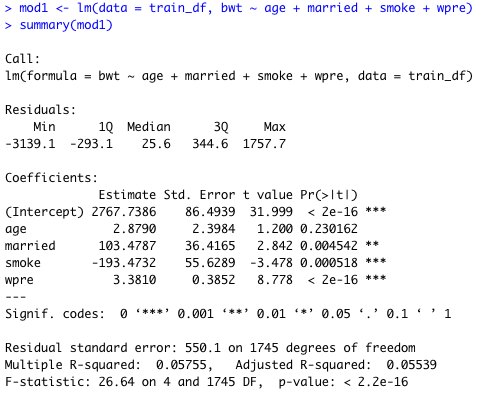
\includegraphics[scale=0.4]{r2_example1.png}
\end{frame}

\begin{frame}{$R^2$: Example in \texttt{R}}
\centering 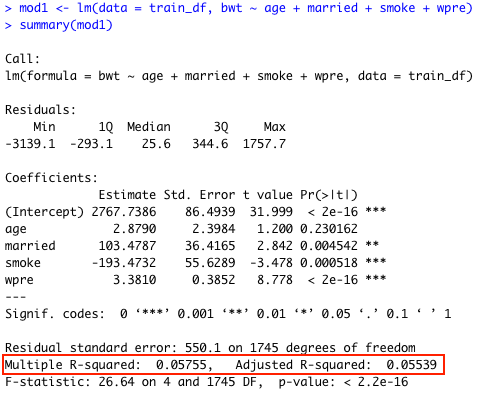
\includegraphics[scale=0.4]{r2_example1_2.png}
\end{frame}

\begin{frame}{$R^2$: Example in \texttt{R}}
\centering 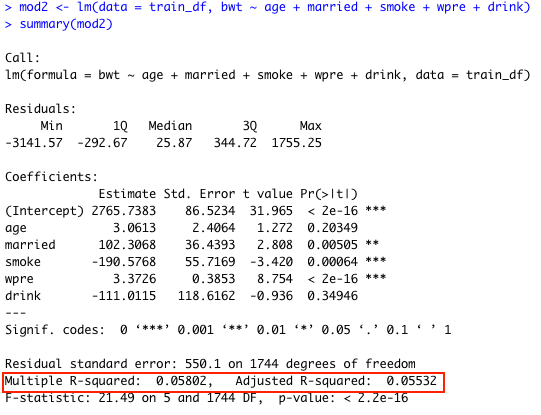
\includegraphics[scale=0.4]{r2_example2.png}
\end{frame}


\begin{frame}{$R^2$: Example in \texttt{R}}
The adjusted $R^2$ from the model including an additional covariate indicating whether or not birth parent drank during pregnancy is 0.05532, while for the smaller model adjusted $R^2$ is 0.05539. These values are very similar, and the larger model with the additional covariate actually has a \textit{lower} adjusted $R^2$ than the smaller model. This suggests that the inclusion of a covariate for drinking will likely not improve prediction accuracy. \pause

\vspace{0.3cm}

\textcolor{blue}{Question:} How would we interpret the multiple $R^2$ value (0.05755) from the model containg covariates for age, marital status, smoking status, and weight prior to pregnancy? \pause

\vspace{0.3cm}

\textcolor{blue}{Answer:} 5.8\% of the variation in child's birthweight is explained by the variation in birth parent's age, marital status, smoking status, and weight prior to pregnancy. 

\vspace{0.3cm}

\small *as we saw qualitatively with our exploratory plot, this is likely not a very good predictive model! We can now back up our plot with a low $R^2$ value, providing quantative evidence that our prediction model needs improvement
\end{frame}
% include slide about comparing multiple predictive models

\subsection{Mean Squared Error}

\begin{frame}{Mean squared error}
We have now seen a measure of prediction accuracy that involves only the training dataset. What can we use to quantify prediction accuracy using our observed and predicted values for our testing dataset?

\vspace{0.3cm}

Intuitively, we can consider quantifying accuracy based on the \textit{difference} between observed and predicted values for each observation. We could then make sure that differences are treated equally regardless of sign (positive or negative), and take the average of these differences across all observations to get a single number, quantifying how far off our predictions are from the truth.  
\end{frame}

\begin{frame}{Mean squared error}
\textcolor{blue}{Mean squared error (MSE):} $\frac{1}{n} \sum_{i = 1}^n (Y_i - \hat{Y}_i)^2$

\vspace{0.3cm} In words: the average of squared differences between observed outcomes $Y_i$ and predicted values $\hat{Y}_i$

\vspace{0.3cm} \pause
The lower our MSE is, the better our predictions. Note that if $Y_i = \hat{Y}_i$ for all observations (our predicted values are the same as our observations), MSE is equal to zero.
\end{frame}

\begin{frame}{MSE: Example in \texttt{R}}
Suppose we are (again) interested in predicting a baby's birthweight based on birth parent's age, marital status, whether or not they smoke during pregnancy, and weight prior to pregnancy. We first divide our data into training and testing data, fit the model on the training data, and then predict the outcomes for the testing data. We include a snippet of code we previously used for this example below.

\vspace{0.3cm}

\begin{figure}
	\centering 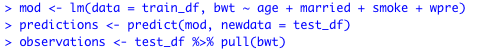
\includegraphics[scale=0.5]{mse1.png}
\end{figure}

\vspace{0.3cm} \pause

\textcolor{blue}{Question:} In \texttt{R}, how would we compute MSE given the objects we have created in the above code snippet?
\end{frame}

\begin{frame}{MSE: Example in \texttt{R}}

\begin{figure}
	\centering 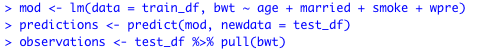
\includegraphics[scale=0.5]{mse1.png}
\end{figure}
\vspace{0.3cm} 

\textcolor{blue}{Question:} In \texttt{R}, how would we compute MSE given the objects we have created in the above code snippet?

\vspace{0.3cm}

\textcolor{blue}{Answer:} 

\vspace{0.3cm}

\texttt{mean((observations - predictions)\^{}2)} 
\end{frame}

\begin{frame}{MSE: Example in \texttt{R}}
Now that we have two different measures of prediction accuracy in our tool-kit, let's apply them both to our question of whether or not including a covariate for drinking in the previous model improves prediction accuracy. We've already done the $R^2$ part in the previous subsection, so we will focus on MSE over the next few slides.

\vspace{0.3cm}
As when computing $R^2$, we first need to fit two separate models to our training dataset.
We then need to obtain predictions for individuals in our \textit{testing} dataset, store our observed outcomes for individuals in our testing dataset, and compute the MSE from both models.
\end{frame}

\begin{frame}{MSE: Example in \texttt{R}}
\begin{figure}
	\centering 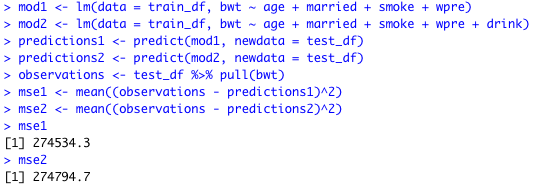
\includegraphics[scale=0.4]{mse2.png}
\end{figure} \pause

\vspace{0.1cm}

Summarizing our results from before, we found that:

\begin{itemize}
	\item Model 1 (no drinking covariate): Adjusted $R^2$ = 0.05539, MSE = 274534.3
	\item Model 2 (drinking covariate): Adjusted $R^2$ = 0.05532, MSE = 274794.7
\end{itemize} \pause

Both MSE and Adjusted $R^2$ indicate that Model 1 is our preferred prediction model, in terms of predictive accuracy. Note that MSE will not always ``agree" with $R^2$. In practice, you may need to decide which quantity you care about more.

\end{frame}

\section{Additional prediction topics}

% is it okay to fit multiple models? yes because prediction not inference
\begin{frame}{How many models can we make?}

You may have heard of \textcolor{orange}{data dredging} or \textcolor{orange}{p-hacking} before, which involves misusing either data selection mechanisms or statistical analyses in order to seek out statistically significant results.

\vspace{0.3cm}


\includegraphics[scale=0.01]{chilipepper.png} In these scenarios, researchers often fit \textit{many} statistical models to their data in an attempt to find a p-value less than 0.05. The problem with this is that when you perform multiple statistical analyses (multiple hypothesis tests), Type I Error rate (the probability that we reject the null hypothesis even though the null is true) can get very large. There are ways to correct for this (typically either setting your hypothesis before data collection and statistical analysis, or doing a \textcolor{orange}{multiple testing} correction for your p-values). 

\vspace{0.3cm}

With prediction, we are not conducting hypothesis tests. We are simply trying to find the ``best" predictive model using the data that we have access to. With inference, running multiple tests (multiple statistical models) on the same dataset may be cause for concern, but with prediction, \textcolor{blue}{we can fit as many models as we want!}

\end{frame}

\begin{frame}{Bias-variance tradeoff 
\includegraphics[scale=0.01]{chilipepper.png}}
With any prediction model we fit, we will have measures of \textcolor{blue}{bias} and \textcolor{blue}{variance}.

\vspace{0.3cm}

\begin{itemize}
	\item \textcolor{blue}{Bias:} how far our predictions are from the truth
	\item \textcolor{blue}{Variance:} how variable our predictions are
\end{itemize}

\vspace{0.3cm} 

Both bias and variance have mathematical experessions (not included here), that lead us to the equation
$$
\text{MSE} = \text{Bias}^2 + \text{Variance}
$$ \pause

In many prediction scenarios (as we saw), we want a predictive model that \textit{minimizes} MSE. Ideally then, we want a model where both bias and variance are small. 
\end{frame}

\begin{frame}{Bias-variance tradeoff 
\includegraphics[scale=0.01]{chilipepper.png}}
Note that we could have two different models that produce predictions with the same MSE, but have very different values for bias and variance:

\vspace{0.3cm}

\begin{itemize}
	\item MSE = $10^2 + 1 = 101$ (Bias = 10, Variance = 1)
	\item MSE = $1^2 + 100 = 101$ (Bias = 1, Variance = 100)
\end{itemize}

\vspace{0.3cm}

Note that to maintain the same MSE, if we increase bias we must decrease variance. Similarly, if we increase variance we must descrease bias. This is called the \textcolor{orange}{bias-variance tradeoff}. When improving upon a prediction model (making a new model with better predictive accuracy), we often have to choose between minimizing bias \textit{or} minimizing variance. \pause

\vspace{0.3cm}

\small In certain scenarios, we may be okay with our predictions having a larger amount of bias in exchange for smaller variances. In some scenarios, we may require \textit{no} bias, and therefore only focus on minimizing variance in our predictions. This will depend on the context of the prediction problem!
\end{frame}

\begin{frame}{Bias-variance tradeoff 
\includegraphics[scale=0.01]{chilipepper.png}}
High variance in a predictive model may come from \textcolor{blue}{overfitting}, or an overly complex model. Interpolation is an extreme example of this, where we have overfit our data so much that each prediction is exactly the same as our observed values.

\vspace{0.3cm}

High bias in a predictive model may come from \textcolor{blue}{underfitting}, where our model is \textit{not complex enough} to adequately capture the observed outcomes in a testing dataset. An example of underfitting would be fitting a simple linear regression model to data where there is clearly a quadratic relationship between $X$ and $Y$ (as we saw in an example earlier in this slide deck).

\end{frame}

% we only have a single training dataset and a single testing dataset, why? - cross validation
\begin{frame}{Cross-validation 
\includegraphics[scale=0.01]{chilipepper.png} }
So far we have only discussed creating a \textit{single} testing and training dataset from our original dataset. This is sometimes done in practice, and is completely justifiable! However, it also common to instead split our original dataset into training and testing datasets \textit{multiple} times, and compute an average measure of prediction accuracy across these multiple training and testing datasets.

\vspace{0.3cm}

\textcolor{blue}{Cross-validation:} The process of creating training and testing datasets many times, over which we compute measures of prediction accuracy. These measures are then averaged to assess predictive model performance.

\vspace{0.3cm}

What bother? By creating many training and testing datasets from the model and averaging across them, cross-validation reduces the variability in our prediction accuracy measures, and therefore gives us a better understanding of what those prediction accuracy measures really are.

\end{frame}

\begin{frame}{Cross-validation 
\includegraphics[scale=0.01]{chilipepper.png} }
What does this look like in practice?

\vspace{0.3cm}

for $j = 1, \dots, k$ times:

\vspace{0.3cm}

\begin{enumerate}
	\item Randomly split the dataset into training (\texttt{train\_df\_j}) and testing (\texttt{test\_df\_j}) data
	\item Fit our model (\texttt{mod\_j}) on the training data set
	\item Obtain predictions (\texttt{predictions\_j}) using the testing dataset 
	\item Compute MSE (\texttt{mse\_j}), or other measures of prediction accuracy, using predictions and observations 
\end{enumerate}

\vspace{0.3cm}

and compute the average MSE across all testing datasets as $\frac{1}{k} \sum_{i = 1}^k \text{MSE}_j$ 

\end{frame}

\begin{frame}{Prediction in Linear Regression: Summary}
By now, you should be able to\dots

\vspace{0.3cm}
\begin{itemize}
	\item Understand and explain the difference between the scientific goals of prediction vs. inference
	\item Be able to compute fitted values in \texttt{R} and by hand
	\item Understand the importance of training vs. testing data, and how to create training and testing datasets in \texttt{R}
	\item Determine the predictive accuracy of a linear regression analysis using $R^2$ and mean squared error (MSE)
	\item Use $R^2$ and MSE to choose a prediction model
\end{itemize}
\end{frame}


\begin{frame}[c]
\centering \huge Any Questions?
\end{frame}

\end{document}